In this chapter, we compute	the flow around randomly-formed aggregates and 
characterize the resulting hydrodynamic forces in a constant-density fluid.
Since the 1980s, there have been numerous models of aggregation, including marine aggregation, based on the random motion of small particulates 
\cite{rosenstock_cluster_1980, witten_diffusion-limited_1981,witten_tenuous_1986,kolb_anisotropic_1987}. To form aggregates, we use two established models: individually-added aggregation and cluster-cluster aggregation, which we describe in detail in \cite{yoo_hydrodynamic_2020}. 
We study the hydrodynamics of flow around a broad sample of the resulting aggregates.
In situ, measurements of oceanic aggregates have shown an approximately linear relationship between the drag and the aggregate diameter \cite{alldredge_situ_1988}. Experimental studies of settling aggregates first focused on inorganic clusters \cite{wiltzius_hydrodynamic_1987} and later considered precisely constructed aggregates \cite{takayasu_determination_1998} and statistical descriptions of broader ensembles \cite{johnson_settling_1996}. 
It was generally found that a linear relation exists between the drag and the square root of the projected area, which allows for the identification of a corresponding settling hydrodynamic radius \cite{johnson_settling_1996, tang_model_2002}.
However, these experimental studies did not allow for a systematic variation of certain parameters and found a range of results depending on the measure used and the exact composition of the aggregates.  Computational studies, in theory, do not have this limitation. Early numerical results were based on rather coarse approximations of aggregates, using point particle approximations \cite{chen_translational_1984}. The accelerated Stokesian dynamics (ASD) approach, which model aggregates as a collection of spheres and accounts for lubrication forces between them, was later developed \cite{brady_stokesian_1988} and used to estimate a hydrodynamic radius for progressively larger aggregates \cite{rogak_stokes_1990,bossis_hydrodynamic_1991}.
In addition to the drag on settling aggregates, the torque on rotating aggregates 
was computed using ASD \cite{binder_structural_2009}. More recently, results were obtained using Lattice-Boltzmann simulations that also considered inertial effects \cite{zhang_direct_2015}. The distribution of internal stresses in rigid aggregates moving in a constant flow, which may result in an aggregate break-up, was also recently studied using the method of reflections  \cite{gastaldi_distribution_2011} and again using ASD  \cite{vanni_accurate_2015}. We develop here 
computational simulations that, in the regime considered, are more flexible and efficient, allowing us to study a greater number of aggregates, resulting in more statistically reliable results. 


\par
While ocean water is density stratified due to temperature or salinity, we begin with simplifying assumptions to understand settling aggregate dynamics. As marine aggregates have fractal structures, it is important to find an appropriate length scale to see a better agreement with their settling speed. We thus consider a homogeneous fluid in this chapter to choose an effective hydrodynamic radius. 



\section{Aggregation Model}
\label{sec_model}

\begin{figure}[ht]
\begin{center}
   \epsfig{figure=./figures/fig_sample_all.pdf,scale=0.7}
\end{center}
\caption{We show typical aggregates as formed by two different methods. Top row: individually-added-aggregates (IAA) containing (a) 50, (b) 100, and (c) 200 cubes. Bottom row: cluster-to-cluster aggregates (CCA) containing (d) 50, (e) 100, and (f) 200 cubes.}
\label{fig_rad_mass}
\end{figure}

To model marine aggregates, we make use of existing models of aggregation where the constituting particles undergo a random walk
\cite{rosenstock_cluster_1980, witten_diffusion-limited_1981,witten_tenuous_1986,kolb_anisotropic_1987}. 
In these models, particles are typically subject to uniform Brownian motion and attach to one another when 
sufficiently close. The resulting aggregates often have a fractal structure characterized by a fractal dimension, $d$. The fractal dimension describes the nature of these complicated objects and may be defined from the relation $N\sim(R_s/l)^d$, where $N$ is the number of particles of length scale $l$ that are part of the aggregate within a sphere of radius $R_s$ \cite{witten_tenuous_1986}. In general, fractal dimensions of aggregate models have been found to range from 1.3 to 3 depending on the exact formation 
mechanism \cite{witten_diffusion-limited_1981, kolb_anisotropic_1987,gmachowski_calculation_2002}. 
Direct observations of marine aggregates have found fractal dimensions ranging approximately from 1.3 to 2.5 \cite{alldredge_situ_1988,jackson_aggregation_1998}.
   
We consider aggregates made of collated cubic particles, as shown in Fig. \ref{fig_rad_mass}. Once formed, we assume that aggregates do not deform, sinter, or break apart \cite{eggersdorfer_multiparticle_2011}.
This is a flexible model that has the advantage of having a
simple external boundary, which will be exploited when we solve for the flow around the aggregate. We generate diffusion-limited aggregates using two different techniques: (1)
individually-added aggregation (IAA) and (2) cluster-to-cluster aggregation (CCA) \cite{witten_tenuous_1986,kolb_anisotropic_1987}. In both methods, each cube has a non-dimensional length, $2$, is aligned with the Cartesian axes, and is centered at a point on a three-dimensional Cartesian lattice restricted to a triply periodic box of period $2P$. The cube centers thus only take values of the form $\{ (2m,2n,2p) \  | m,n,p \in \mathbb{Z}, -P<m,n,p\leq P \}$. 


Typically, the IAA method gives a more compact form of aggregates, with dimension $\sim 2.56$, than the CCA case, which has dimension $\sim 1.79$ \cite{witten_diffusion-limited_1981, kaye_random_2008}. More details regarding the analysis of aggregation formations can be found \cite{yoo_hydrodynamic_2020}.


\par 
To characterize the size of each aggregate, we define the dimensionless gyration radius, $R'_g$, also known as the root-mean-square radius, as
\begin{equation}
{R'}_g  = \sqrt{\frac{1}{NC} \sum_{i=1}^{NC} \| \vec{x}_i - \vec{x}_{cm} \|^2},
\label{eq_Rg}
\end{equation}
and the maximum radius of the aggregate, $R'_m$, is defined as the
maximum of the distances between the center of each of its constituting cubes, $\vec{x}_i$, and the center of
mass, $\vec{x}_{cm}$, to which we add one to account for the size of an individual cube,
\begin{equation}
{R'}_m = 1+ \max_{i = 1, \cdots, NC} \| \vec{x}_i - \vec{x}_{cm} \|,
\label{eq_Rm}
\end{equation}
where $NC$ is the number of cubes in the aggregate.
We obtain the center of mass of the aggregate, $\vec{x}_{cm}$, by taking mean values of each element of $\vec{x}_i$ for $i = 1, \cdots, NC$.
Note that most experimental studies use the projected area method to describe the size of an aggregate. However, since this project is done computationally, which has more freedom than physical experiments, we choose to use those formulations (\ref{eq_Rg}) and (\ref{eq_Rm}) without reduction of dimension.
We will later show the results of different forces acting on the aggregates and examine which measurement captures better characteristics.

%
%--------------------------------------------------------
\section{Derivation of single- and double-layer potentials}
We introduced the equation, (\ref{eq_BIE_onS}), as a solution form to the Stokes equations in chapter \ref{ch:intro}. As we have a solid boundary surface of a marine aggregate model, we are able to use a simplified version of the fundamental solution. We are interested in solving for the flow at points $\vec{x}_0$ in the fluid domain extending to infinity and external to the surface, $S$, of an aggregate, as shown in Figure \ref{fig_cube10}.
We take advantage of the linearity of the Stokes equations and express the velocity as a boundary integral over the surface of the aggregate \cite{pozrikidis_boundary_1992, stakgold_boundary_2000}. 
The resulting Fredholm integral formulae have the advantage of involving computations in two dimensions only, despite the three-dimensionality of the system.
For solid objects, one may obtain two different  Fredholm integral formulae. We introduce both formulations in the remainder of this section and compare them in the following section. 
\subsection{Single-layer potential (SLP)}
We first derive the velocity with the single-layer potential alone.
The solid boundary condition allows us to express its velocity as 
\begin{equation}
	\vec{u}_s \left( \vec{x} \right) 
	= \vec{U}_a + \vec{\Omega} \times \left( \vec{x} - \vec{x}_{cm} \right),
	\label{eq_solidbody}
\end{equation}
where $\vec{U}_a$ and $\vec{\Omega}$ are constant translational and angular velocities, respectively. Without loss of generality, we conveniently choose a zero center of mass, $\vec{x}_{cm} = \vec{0}$, for this derivation.
Substituting the solid object velocity, equation (\ref{eq_solidbody}), into the double-layer potential in equation (\ref{eq_BIE}) shows that 
\begin{align}
	\int_S
	\left( \vec{U}_a + \vec{\Omega} \times \vec{x} \right)
	 \cdot  \bar{\bar{K}}(\vec{x},\vec{y})  
	\cdot \hat{n} ( \vec{x})
	\ \text{d}S(\vec{x})
    \nonumber \\
	= 
	\int_S
	\vec{U}_a
	 \cdot  \bar{\bar{K}}(\vec{x},\vec{y})  
	\cdot \hat{n} ( \vec{x})
	\ \text{d}S(\vec{x})
     + 	
	\int_S
	\left(  \vec{\Omega} \times \vec{x} \right)
	 \cdot  \bar{\bar{K}}(\vec{x},\vec{y})  
	\cdot \hat{n} ( \vec{x})
	\ \text{d}S(\vec{x})
	\label{eq_solid_motion_dlp}
\end{align}
% We consider two flows, $\vec{U}_a$ and $\vec{\Omega}$, separately. 
The first integral of the right-hand side of the equation (\ref{eq_solid_motion_dlp}) can be re-written as 
\begin{equation}
	\vec{U}_a \cdot
	\int_S
	  \bar{\bar{K}}(\vec{x},\vec{y})  
	\cdot \hat{n} ( \vec{x})
	\ \text{d}S(\vec{x}),
	\label{eq_solid_motion_dlp_Ua}
\end{equation}
since the translational velocity, $\vec{U}_a$, is constant. 
For the flow around (outside) and on the solid object, Pozrikidis provides a useful identity \cite{pozrikidis_boundary_1992} (page 21, equation (2.1.12))
\begin{align}
	\int_S  \bar{\bar{K}}(\vec{x},\vec{y}) \cdot \hat{n} ( \vec{x})
	\ \text{d}S(\vec{x})
	=
	 \begin{cases}
	 \bar{\bar{0}} & \text{ if } \vec{y} \in \mathbb{R}^3  \setminus  \left( S \cup {\text{inside of aggregate}}\right) 	\\ 
	 - 4\pi \bar{\bar{I}} & \text{ if } \vec{y} \in S 
	 \end{cases}.
	\label{eq_dlp_identity1}
\end{align}
Then, including the velocity $\vec{U}_a$, we get
\begin{align}
	\vec{U}_a \cdot
	\int_S  \bar{\bar{K}}(\vec{x},\vec{y}) \cdot \hat{n} ( \vec{x})
	\ \text{d}S(\vec{x})
	=
	 \begin{cases}
	 \vec{0}& \text{ if } \vec{y} \in \mathbb{R}^3  \setminus \left( S \cup {\text{inside of aggregate}}\right) 	\\ 
	 - 4\pi \vec{U}_a  & \text{ if } \vec{y} \in S 
	 \end{cases}.
	\label{eq_dlp_Ua}
\end{align}
% Applying these values to the representation formulae, equation(\ref{eq_BIE}) and (\ref{eq_BIE_onS}), allows us to remove the double-layer potential.
\par 
The second integral in equation (\ref{eq_solid_motion_dlp}) can be evaluated with the following identity, from \cite{pozrikidis_boundary_1992},
using Einstein (summation) notation, 
\begin{align}
	\varepsilon_{i \ell m}
	\int_S x_{\ell} \ T_{mjk}(\vec{x},\vec{y})  \ n_{k} ( \vec{x})
	\ \text{d}S(\vec{x})
	 = 
	 \begin{cases}
	  \vec{0}
	  & \text{ if } \vec{y} \in \mathbb{R}^3  \setminus  	\left( S \cup {\text{inside of aggregate}}\right) \\ 
	 - 4\pi \ \varepsilon_{i \ell j} \ x_{\ell}
	 & \text{ if } \vec{y} \in S 
	 \end{cases},
	\label{eq_dlp_identity2}
\end{align}
where $\varepsilon_{i \ell m}$ is the Levi-Civita permutation symbol.  
Multiplying both sides by the angular velocity, $\Omega$, in equation (\ref{eq_dlp_identity2}), we get 
\begin{align}
	&
	\int_S
	\left( \vec{\Omega} \times \vec{x} \right)
	 \cdot  \bar{\bar{K}}(\vec{x},\vec{y})  
	\cdot \hat{n} ( \vec{x})
	\ \text{d}S(\vec{x})
	 = 
	\int_S 
	\left(  \varepsilon_{i \ell m} \ \Omega_{i} x_{\ell} \right) \ 	T_{mjk}(\vec{x},\vec{y})  \ n_{k} ( \vec{x})
	\ \text{d}S(\vec{x})
	\nonumber \\
	\nonumber \\
 	& = 
 	\begin{cases}
 	  \vec{0}
 	 &  \\ 
 	- 4\pi \ \varepsilon_{i \ell j}\  \Omega_{i} \ x^0_{\ell}
 	& 
 	\end{cases}
	= \begin{cases}
 	  \vec{0}
 	 & \text{ if } \vec{y} \in \mathbb{R}^3  \setminus  
	 \left( S \cup {\text{inside of aggregate}}\right)
	  \\ 
 	- 4\pi \left(  \Omega \times \vec{y} \right)
 	& \text{ if } \vec{y} \in S.
 	\end{cases}
	\label{eq_dlp_Omega}
\end{align}
We now combine two equations, (\ref{eq_dlp_Ua}) and (\ref{eq_dlp_Omega}),
\begin{equation}
	\int_S \vec{u} ( \vec{x}) \cdot \bar{\bar{K}}(\vec{x},\vec{y}) \cdot \hat{n} ( \vec{x})
	\ \text{d}S(\vec{x})
	 = 
	 \begin{cases}
	  \vec{0}& \text{ if } \vec{y} \in \mathbb{R}^3  \setminus \left( S \cup {\text{inside of aggregate}}\right)
	  \\ 
	 - 4\pi \vec{u}(\vec{y}) & \text{ if } \vec{y} \in S 
	 \end{cases}.
	\label{eq_dlp_val_out}
\end{equation}
When the point $\vec{y}$ is strictly outside of the aggregate surface, $S$,
 \begin{equation}
    \vec{u}(\vec{y}) = - \frac{1}{8 \pi \tilde{\mu}} \int_S  \vec{f}(\vec{x}) \cdot \bar{\bar{G}}(\vec{x},\vec{y}) \ \text{d}S(\vec{x}) ,
 \label{eq_slp}
 \end{equation}
 only the single-layer potential term.
For evaluation points on the surface $S$, 
$\vec{y} = \vec{x}_s \in S$, 
since the double-layer potential is $- 4 \pi \vec{u}(\vec{x}_s)$, when we substitue into equation (\ref{eq_BIE_onS}), 
we obtain exactly the same equation (\ref{eq_slp}). This implies that the single-layer potential formula is continuous across the boundary surface $S$.
To analyze the force and torque, we use the stress $\vec{f}$ in equation (\ref{eq_slp}) as
\begin{equation}
	\vec{F} = \int_s \vec{f}(\vec{x}) \  \text{d}S(\vec{x}) \hspace{1 cm} \text{ and } \hspace{1 cm}   \vec{Q} = \int_s (\vec{x} - \vec{x}_{cm}) \times \vec{f}(\vec{x})  \ \text{d}S(\vec{x}).
	\label{eq_total_FT}
\end{equation}
 where $\vec{F}_o$ and $\vec{Q}_o$ represent the total force and torque, respectively, acting on the aggregate surface $S$.
%
% Note that the single-layer potential is continuous across the surface boundary as long as the surface is smooth in general. The following theorem is cited from \cite{kress_linear_2014}.
% \begin{thm}
% 	Let $S$ be of class $C^2$ and $f \in C(S)$. Then the single-layer potential $u$ with density $f$ is continuous throughout $\mathbb{R}^m$. On the boundary $S$, we have
% 	\begin{equation*}
% 		u(x) = \int_S f(y) G(x,y) \ \text{d}S(y), \ \ \ x \in S,
% 	\end{equation*}
% 	where the integral exists as an improper integral.
% 	\label{eq_thm1}
% \end{thm}
% Although our aggregate model is not smooth overall with edges and corners, the idea of theorem (\ref{eq_thm1}) is valid for our approximation since we only use the boundary integral equations on the center of each discretized square face. We discuss details in the next chapter.

\subsection{Double-layer potential (DLP)}
The second approach we can take is removing the single-layer potential. 
To derive the double-layer potential formulation, we consider a complimentary flow $\vec{u}_c$ 
% (not to be confused with the derivative prime notation) 
for the points \textit{inside} of the aggregate surface boundary $S$, having the same force on the boundary as $\vec{u}$. More specifically, the velocity $\vec{u}$  has the representation form, equation (\ref{eq_BIE}) and the complimentary flow $\vec{u}_c$ has the same stress, $\vec{f}$, on the boundary as $\vec{u}$. Before we proceed, we shall justify the existence of the complimentary flow.
The new flow $\vec{u}_c$ can be found when the velocity $\vec{u}$ on the boundary satisfies
\begin{equation}
 	\int_S \vec{u}(\vec{x}) \cdot \hat{n} \ \text{d}S(\vec{x})=0. 
	\label{eq_dlp_constraint}
\end{equation}
This condition is taken from \cite{pozrikidis_boundary_1992}.
This can be fulfilled with our problem due to the continuity equation, $\nabla \cdot \vec{u}= 0$, and the divergence theorem.
By the conservation of mass, we can say
\begin{equation}
 	\int_V  \nabla \cdot \vec{u}(\vec{x}) \ \text{d}V (\vec{x}) 
		=0. 
	\label{eq_constraint_v}
\end{equation}
By the divergence theorem, we have
\begin{equation}
	\int_V  \nabla \cdot \vec{u}(\vec{y}) \ \text{d}V (\vec{y})   = 
\int_{S } \vec{u}(\vec{x}) \cdot \hat{n} \ \text{d}S(\vec{x})
+ \int_{S_f} \vec{u}(\vec{x}) \cdot \hat{n} \ \text{d}S(\vec{x})=0,
\label{eq_div}
\end{equation}
where $S_f$ is the surface of the control volume of the fluid, $V$, surrounding the solid particle. See Figure \ref{fig_dlp_volume}.
Note that the fluid volume $V$ is strictly outside of the aggregate boundary $S$. 
\begin{figure}[h]
	\begin{center}
		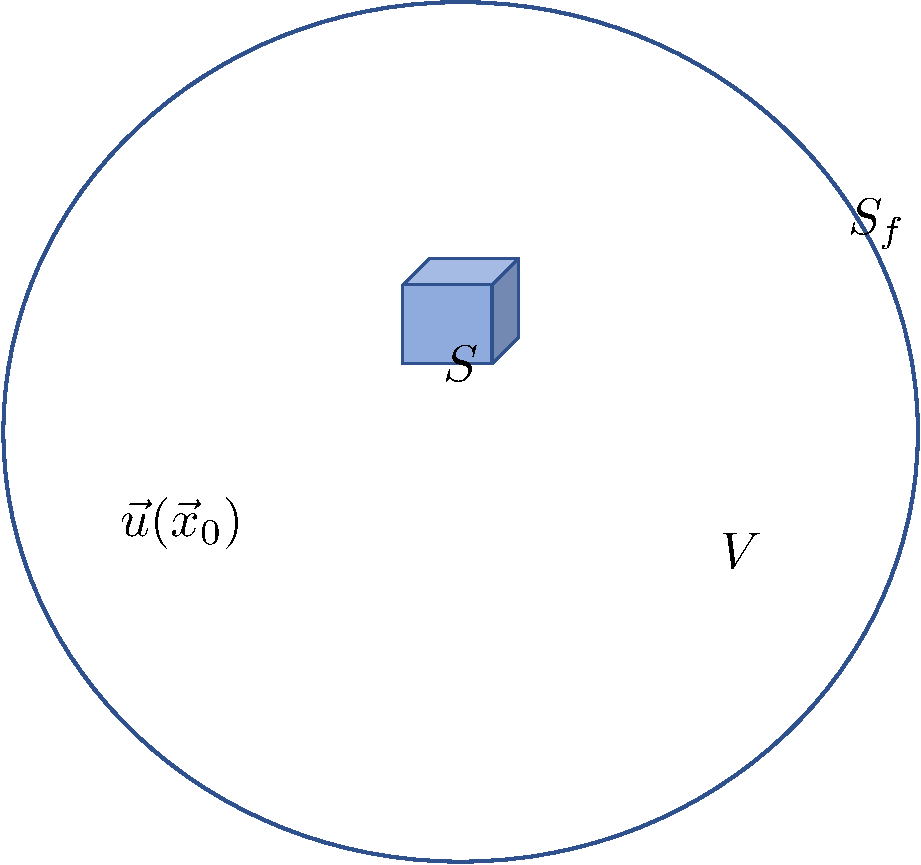
\includegraphics[scale=0.4]{./figures/fig_dlp_volume}
		\vspace{0.5cm}
	\caption{Schematic of the control volume and its surface.}
	\label{fig_dlp_volume}
\end{center}
\end{figure}
The control volume could be a large sphere with its radius $r_f$. Then the velocity $\vec{u}$ on $S_f$ approaches zero with the order of $\mathcal{O}(1/r_f)$ and its associated stress tensor decays with the rate $\mathcal{O} (1/r_f^2)$. Once the surface integral on $S_f$ in equation (\ref{eq_div}) becomes zero, it implies that
\[
\int_{S} \vec{u}(\vec{x}) \cdot \hat{n} \ \text{d}S(\vec{x}) = 0.
\]
%  It also means that the net force on the surface $S$ is zero. 
Now, we have a complementary flow $\vec{u}_c$.  By the Lorentz reciprocal identity, any two flows having the same force on the boundary satisfy
% pozrikidis equation (2.3.26)
\begin{equation}
	\int_{S}  \vec{f}(\vec{x}) \cdot \bar{\bar{G}}(\vec{x},\vec{x}_o) \ \text{d}S(\vec{x})  
	- \tilde{\mu} \int_S
	  \vec{u}_c(\vec{x}) \cdot  \bar{\bar{K}}(\vec{x},\vec{x}_o) 
	  \cdot \hat{n} ( \vec{x})
	  \ \text{d}S(\vec{x})
	  =0,
	  \label{eq_comple_identity}
\end{equation}
Substituting equation (\ref{eq_comple_identity}) into the representation formula, equation (\ref{eq_BIE}), we obtain a flow
\begin{align}
   \vec{u}_{dl}(\vec{y}) & =
	\frac{1}{8 \pi } \int_S  
	% \left( \vec{u}(\vec{x})  - \vec{u'}(\vec{x})  \right)
	\vec{\psi}(\vec{x})
	\cdot  \bar{\bar{K}}(\vec{x},\vec{y})  
	\cdot \hat{n} ( \vec{x})
	\ \text{d}S(\vec{x}),
\label{eq_BIE_for_dlp}
\end{align}
where $
	\vec{\psi}(\vec{x}) =    \vec{u}(\vec{x})  - \vec{u}_c (\vec{x})$.
When $\bar{\bar{T }}$ is a Green's function for an infinite flow, the velocity (\ref{eq_BIE_for_dlp}) satisfies the Stokes equation with any choice of $\vec{\psi}(\vec{x}) $.
\par
 % Thus, the velocity formula with only the double-layer potential would be valid for the zero net force model.

Due to our constraint to derive the equation (\ref{eq_BIE_for_dlp}), the double-layer potential formula, $\vec{u}_{dl}$ is only valid for a particle that has a force- and torque-free body, such as a swimming microorganism.
For other solid-body models, finite non-zero net force and torque models, the velocity we would like to find, $\vec{u}$, does not capture the force and torque on the surface $S$ accurately, i.e., 
\begin{equation}
\vec{u}_{dl}(\vec{y}) = \vec{u}(\vec{y}) 
- \frac{1}{8 \pi \tilde{\mu} }\vec{F}_o \cdot \bar{\bar{G}}(\vec{x}_{0}, \ \vec{x}_{cm})
- \frac{1}{8 \pi \tilde{\mu} } \frac{\vec{Q}_o \times  (\vec{y}   - \vec{x}_{\text{cm}} ) }{\| \vec{y}   - \vec{x}_{\text{cm}} \|^3 }.
\label{eq_v_dlp}
\end{equation}
For the double-layer potential formula, we define the total force and torque as
\begin{equation}
 \vec{F}_o
  = \frac{\tilde{\mu}}{L} \int_S \vec{\psi}(\vec{x}) \  \text{d}S(\vec{x})
 % = \frac{\tilde{\mu}}{L} \int_S  \vec{\psi}( \vec{x}) \ \text{d}S(\vec{x}),
 \label{alpha_dl}
 \end{equation} 
 and
 \begin{equation}
 \vec{Q}_o 
 = \frac{\tilde{\mu}}{L} \int_S (\vec{x} - \vec{x}_{cm}) \times \vec{\psi}(\vec{x})  \ \text{d}S(\vec{x})
 \label{omega_dl}
 \end{equation}
%
We multiply by $\tilde{\mu} / L$ to consider the same physical meaning as the stress vector, $\vec{f}$, as we found the forces using the single-layer potential case, equations (\ref{eq_forcebal}) and (\ref{eq_total_Torque_slp}).
Note that equation (\ref{eq_v_dlp}) implies that the net force and torque associated to the velocity $\vec{u}_{dl}$ are zero.
The second and third terms in equation (\ref{eq_v_dlp}), denoted by $\vec{u}_F$ and $\vec{u}_Q$, respectively, are a solution to the Stokes equations, except at the center of mass of the solid particle, $\vec{x}_{cm}$.
The flow $\vec{u}_F$ is the velocity at a point $\vec{y}$ generated by the point force with strength $\vec{F}_0$ at $\vec{x}_{cm}$. 
In the same manner, the flow $\vec{u}_Q$ represents the velocity induced by the vorticity associated with the flow $\vec{u}_F$.
With those two extra terms, Mikhlin 1957, p.172 \cite{smithies_integral_1959} and Power \& Miranda 1987 \cite{power_second_1987} introduced the following double-layer potential formula,
\begin{equation}
\vec{u}(\vec{y}) = \int_S
\vec{\psi}(\vec{x}) \cdot  \bar{\bar{K}}(\vec{x},\vec{y})  \ \text{d}S(\vec{x}) + 
\frac{1}{8 \pi \tilde{\mu} }\vec{F}_o \cdot \bar{\bar{G}}(\vec{x}_{0},\vec{x}_{cm})
+\frac{1}{8 \pi \tilde{\mu} } \frac{\vec{Q}_o \times  (\vec{y}   - \vec{x}_{cm} ) }{\| \vec{y}   - \vec{x}_{cm} \|^3 },
 \label{eq_BI_DL}
\end{equation}
where $ \bar{\bar{K}}(\vec{x},\vec{y})$ combines the stresslet and normal vector,
% where
\begin{equation*}
	\bar{\bar{K}}(\vec{x},\vec{y})
	= \frac{1}{8 \pi} \bar{\bar{K}}(\vec{x},\vec{y})  \cdot \hat{n}(\vec{x}),
\end{equation*}
for any points outside of the solid particle surface, $S$.

\par
Unlike the single-layer potential, the double-layer potential formula is not continuous across the surface, $S$.
We thus consider another velocity expression on the aggregate boundary surface with a jump condition,
\begin{equation}
\vec{u}(\vec{x}_s) = -\frac{1}{2} \vec{\psi}(\vec{x}_s) 
+\int_S  \vec{\psi}(\vec{x})  \cdot \bar{\bar{K}} (\vec{x},\vec{x}_s) \ \text{d}S(\vec{x}) 
+\frac{1}{8 \pi \tilde{\mu} } \vec{F}_o \cdot \bar{\bar{G}}(\vec{x}_{s},\vec{x}_{cm})
+\frac{1}{8 \pi \tilde{\mu} } \frac{\vec{Q}_o \times  (\vec{x}_s   - \vec{x}_{\text{cm}} ) }{\| \vec{x}_s  - \vec{x}_{\text{cm}} \|^3 },
\label{eq_BI_DL_on}
\end{equation}
for the points on the surface, $\vec{x}_s \in S$.
%-----------DIMENSIONAL ANALYSIS---------------------------------------------------------------
\section{Non-dimensionalization}
\label{section3}
For the convenience of further study, we write all equations in non-dimensional form using the following parameters:
\begin{equation}
\vec{x} = R_a\vec{x}', 
\ \
 \vec{u} = U_s \vec{u'},
 \ \ 
  \vec{f} = \frac{\tilde{\mu} U_s}{R_a} \vec{f'},
  \ \ 
  \vec{\psi} = U_s \vec{\psi}',
  \ \ 
  \vec{F_o} = \tilde{\mu} U_s R_a \vec{F_o}',
  \ \
  \vec{Q_o} = \tilde{\mu} U_s R_a^2 \vec{Q_o}'.
\label{eq_nonD}
\end{equation}
We use the values presented in Chapter 1, as we derived the Reynolds number (\ref{eq_Re}). 
Then the system of equations becomes
\begin{align}
    -\nabla' P_d' +  \nabla'^2 \vec{u}'  = \vec{0}
	\label{eq_momentum_noD}
	\\
    \nabla' \cdot \vec{u}' = 0,
	\label{eq_conti_noD}
\end{align}
where we define the dynamic pressure as 
$P_d(\vec{x}) =  P(\vec{x}) + \rho g \hat{k} \cdot \vec{x}$.
Equation (\ref{eq_solidbody}), used in both the single-layer and double-layer formulations, is thus non-dimensionalized as 
\begin{equation}
  \vec{u}'(\vec{x}'_s) = \frac{\vec{U}_a}{U_s} +  \frac{\vec{\Omega}R_a}{U_s} \times (\vec{x}'_s - \vec{x}'_{cm}) = \vec{U}'_a +  \vec{\Omega}' \times (\vec{x}'_s - \vec{x}'_{cm})
  \label{eq_solidbody_nonD}
\end{equation}
Furthermore, dimensionless forms of the single-layer potential formula for the velocity at a point outside of the surface $S$ is 
\begin{equation}
    \vec{u'}(\vec{y}') =
	- \frac{1}{8 \pi}
	\int_{S'}  \vec{f'}(\vec{x}') \cdot \bar{\bar{G'}}(\vec{x}', \ \vec{y}') \ \text{d}S'(\vec{x}').
    \label{eq_BI_sl_ND}
\end{equation}
% Although $\vec{y}$ represents a point in the fluid, equation (\ref{eq_BI_sl_ND}) is also valid for a point on the surface, $\vec{x}_s$.
\par
The equations for the non-dimensional force and angular velocity, given dimensionally in equation (\ref{eq_total_FT}), become
\begin{align}
\vec{F}' =  \vec{F} \frac{1}{\tilde{\mu} U_s R_a}  =  \int_{S'} \vec{f}'(\vec{x}') \  \text{d}S'(\vec{x}')  
\label{eq_forcebal} 
\\  
 \vec{Q}' = \vec{Q} \frac{1}{\tilde{\mu} U_s R_a^2} =  \int_{S'} (\vec{x}' - \vec{x}'_{cm}) \times \vec{f}'(\vec{x}')  \ \text{d}S'(\vec{x}').  \label{eq_torquebal} 
\end{align}
 We also make dimensionless the double-layer potential in a similar manner, 
 \begin{equation}
 \vec{u}(\vec{y}') = \int_{S'}
 \vec{\psi'}(\vec{x}') \cdot  \bar{\bar{K'}}(\vec{x}', \ \vec{y}')  \ \text{d}S' (\vec{x}') + \vec{F'}_o \cdot \bar{\bar{G'}}(\vec{x}'_{0},\vec{x}'_{cm})
 +\frac{1}{8 \pi} \frac{\vec{Q'}_o \times
 (\vec{y}'   - \vec{x}'_{\text{cm}} ) }{\| \vec{y}'   - \vec{x}'_{\text{cm}} \|^3 },
  \label{eq_BI_DL_noD}
 \end{equation}
 for points outside of $S$, and
 \begin{align}
 \vec{u}(\vec{x}'_s) 
 & =  -\frac{1}{2}\vec{\psi'}(\vec{x}'_s)
 \nonumber  \\
&+  \int_{S'}
 \vec{\psi'}(\vec{x}') \cdot  \bar{\bar{K'}}(\vec{x}', \ \vec{x}'_s)  \ \text{d}S' (\vec{x}') + \vec{F'}_o \cdot \bar{\bar{G'}}(\vec{x}'_{s},\vec{x}'_{cm})
 +\frac{1}{8 \pi} \frac{\vec{Q'}_o \times
 (\vec{x}'_s   - \vec{x}'_{\text{cm}} ) }{\| \vec{x}'_s   - \vec{x}'_{\text{cm}} \|^3 },
  \label{eq_BI_DL_jump_noD}
 \end{align}
 The non-dimensional point-force and torque, given dimensionally in equation (\ref{alpha_dl}) 
 become
 \begin{eqnarray}
  \vec{F}' &=&  \int_{S'}  \vec{\psi}'( \vec{x}') \ \text{d}S(\vec{x}')  
 \label{alpha_dl_nonD} \\
  \vec{Q}' &=&  \int_{S'}  \vec{\psi}'(\vec{x}')  \cdot  (\bar{\bar{\bar{\epsilon}}} \cdot \vec{x}' )  \ \text{d}S(\vec{x}') \, .
 \label{omega_dl_nonD}
 \end{eqnarray}

\section{Numerical methods}
\label{sec:numerical}
When solving for the velocity field exterior to a solid object or an aggregate, one may either 
prescribe the translation velocity,  $ \vec{U}'_a$, and angular velocity, $ \vec{\Omega'}$, of the object 
or prescribe 
the total force and torque. 
We found the analysis easier to perform when setting $\vec{U}'_a$ and $\vec{\Omega}'$ to known values, providing us with the velocity on the surface of the object via equation (\ref{eq_solidbody_nonD}). We thus know 
 $\vec{u}'$ on the left-hand-side of equations (\ref{eq_BI_sl_ND}) and (\ref{eq_BI_DL_jump_noD}). Provided we can evaluate the surface integrals, we may then solve for the unknown stress vector, $\vec{f}'$, or density, $\vec{\psi}'$, respectively. Once these are found, we can evaluate the velocity of the fluid at any point exterior to the aggregate using equations (\ref{eq_BI_sl_ND}) or (\ref{eq_BI_DL_noD}) and compute the force and torque via equations (\ref{eq_forcebal}) and (\ref{eq_torquebal}), or equations  (\ref{alpha_dl_nonD}) and (\ref{omega_dl_nonD}).

 \par
 Because we consider aggregates that are composed of cubic particles, their surface is simply a collection of squares.
 In both the single and double-layer potential approach, we impose a velocity at the center of each square on the surface, $\vec{x}_{sq,i}$, where $i = 1,2, \cdots, N_f$, with $N_f$ denoting the total number of square faces of an aggregate. We thus need to compute integrals of the form
 \begin{equation}
 \vec{I}(\vec{x}'_{sq,i}) = \int_{S'} \vec{q}'(\vec{x}') \cdot {\bar{\bar{J}}} (\vec{x}', \vec{x}'_{sq,i}) \ \text{d} S'(\vec{x}').
 \label{eq_pre_discretize}
 \end{equation}
 Here, $\vec{q}$ represents either $\vec{f}$ or $\vec{\psi}$, and $\bar{\bar{J}}$ stands for either $\bar{\bar{G}}$ or $\bar{\bar{\bar{K}}}\cdot\hat{n}$, depending on if the single or double-layer method is used, respectively.  To allow an exact analytic computation of the integrals, we assume that on the $k$th square face, the vector $\vec{q}'(\vec{x}') = \vec{q}'_k$ is constant, for $k = 1, 2, \dots, N_f$.
 The surface integrals over the entire aggregate may then be discretized as
 \begin{equation}
 \vec{I}(\vec{x}'_{sq,i})  =   \sum_{k=1}^{N_f}  \vec{q}'_k   \int_{S'_{k}} \bar{\bar{J}}(\vec{x}',\vec{x}'_{sq,i}) \ \text{d}S'(\vec{x}') = \sum_{k=1}^{N_f} \vec{q}'_k   \ \bar{\bar{\Pi}}'_{i,k}.
 \label{eq_discretized}
 \end{equation}
 where the coefficients $\bar{\bar{\Pi}}'_{i,k}$ are constant. These constants may be computed analytically, and the corresponding formulae are given in Appendix A.
  This discretization is equivalent to using a two-dimensional mid-point rule to estimate the integrals.  Equation (\ref{eq_discretized}) is linear in $\vec{q}'_k$, resulting in a dense linear system of 3$N_f$ equations for each of the $N_f$ three-dimensional unknown vectors $\vec{q}'_k$ (either the stress vector or the density). 
 \par
 We note that the numerical method presented here describes the fluid flow around a single aggregate but a similar procedure can be employed to determine the flow exterior to several aggregates. Each aggregate then has its own translation and angular velocity vectors, as well as its own force and torque. In that case, it is more natural to set the force and torque on each particle, using equations (\ref{eq_forcebal}) and (\ref{eq_torquebal}) or equations  (\ref{alpha_dl_nonD}) and (\ref{omega_dl_nonD}), and then solve for the translation and angular velocities, adding two vector equations per aggregate to the linear system.
 \par
 We now discuss specific features of the single- and double-layer potential methods. For the single-layer potential, we have $\bar{\bar{J}}(\vec{x}',\vec{x}'_k) = \bar{\bar{G}}(\vec{x}',\vec{x}'_k)$, and $\vec{q}'_k = \vec{f}'_k$. 
 In that case, the $3N_f \times 3N_f$ linear system obtained is not full rank. Stress vectors are only found up to a constant multiple of the local normal vectors since a stress vector given by a constant multiple of the local normals results in a zero velocity at the interface and a zero net force and torque. To obtain a unique solution, we add an equation enforcing that
 \begin{equation}
 \sum_{k=1}^{N_f} \vec{f}'_k \cdot \hat{n}_k = 0,
 \label{eq_constraint}
 \end{equation}
 where $\hat{n}_k$ is the outer normal on each face. The resulting $(3N_f +1)\times 3N_f$ system has a unique solution vector $\vec{f}'_k$. 
 \par
 For the double-layer potential, the unknown density, $\vec{\psi}'_k$, is found using the same discretization (\ref{eq_discretized}) applied to equation (\ref{eq_BI_DL_jump_noD}), resulting in a system with no rank deficiency. However, the values of the total force and torque terms must be solved simultaneously with the unknown density, resulting in a slightly larger system of size $3(N_f+2)\times 3(N_f+2)$. These additional  equations, (\ref{alpha_dl_nonD}) and (\ref{omega_dl_nonD}), are discretized as,
 \begin{eqnarray}
 0 \ &=& \
 \int_{S'}  \vec{\psi}'( \vec{x}')  \ \text{d}S'(\vec{x}') -  \vec{F}' \ = \
A' \sum_{k=1}^{N_f} \vec{\psi}'_k   -  \vec{F}', \label{eq_disc_dlF} \\
0 \ &=& \
  \int_{S'}  \vec{\psi}' ( \vec{x}') \cdot  (\bar{\bar{\bar{\epsilon}}} \cdot \vec{x}' )  \ \text{d}S'(\vec{x}')
 - \vec{Q}'
\ = \
 A' \sum_{k=1}^{N_f} \vec{\psi}'_k   \cdot \bar{\bar{\bar{\epsilon}}}  \cdot  \vec{x}'_k   - \vec{Q}' \label{eq_disc_dlQ}
 \end{eqnarray}
where $A' = 4$ is the non-dimensional area of each square.
\begin{figure}[ht]
	\begin{center}
	  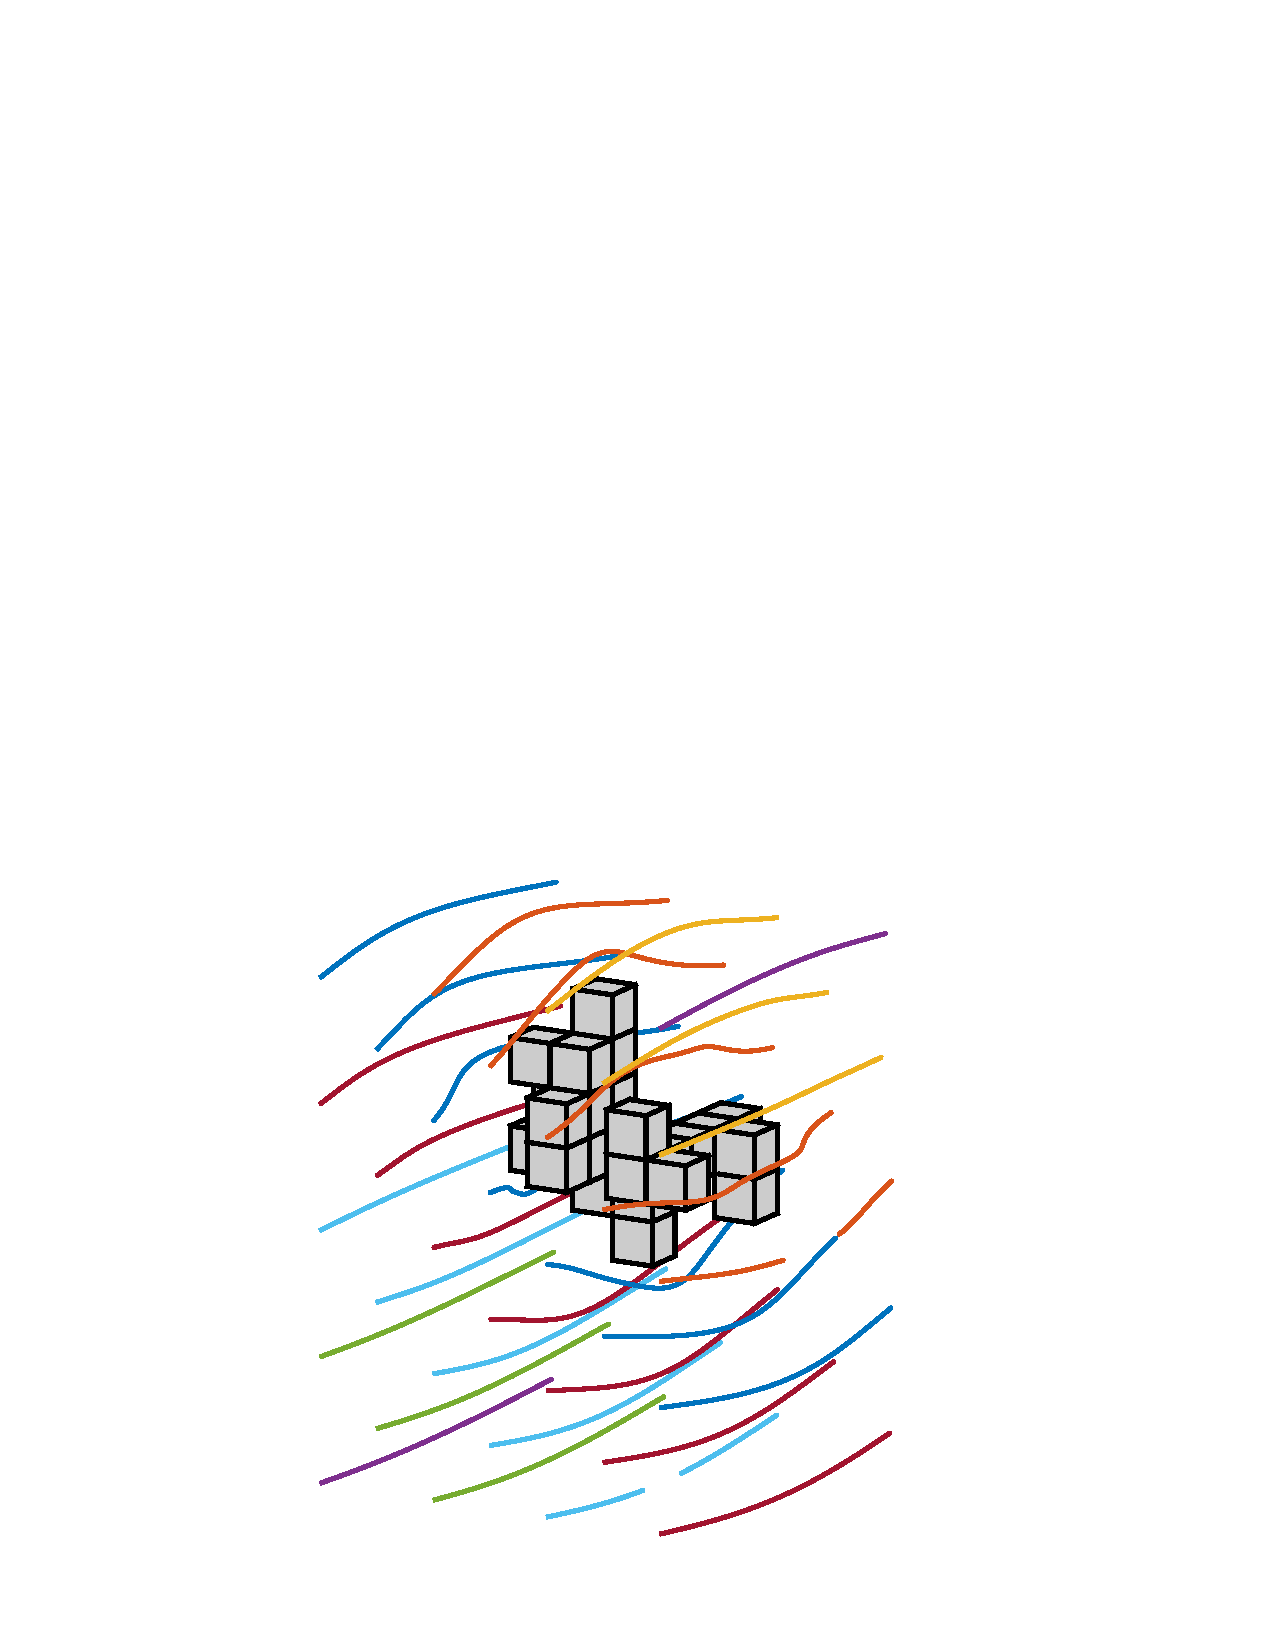
\includegraphics[scale = 0.4]{./figures/fig_streamlines25_fig120.pdf}
	 \end{center}
	\caption{Sample streamlines of flow past a 20-cube aggregate. The aggregate is assumed to move horizontally, into the page and to the right.
	}
	\label{fig_stream}
	\end{figure}
	
	In Fig. \ref{fig_stream}, we present sample streamlines computed with this numerical method. Here, we show results obtained with the single-layer potential method where the aggregate is assumed to move horizontally with $\vec{U}'_a = (1,0,0)$ and $\vec{\Omega}' = (0,0,0)$. The double-layer potential would give results that are visually identical. Once the velocity was computed, the streamlines were obtained by performing a second-order Runge-Kutta time integration.  The streamlines, computed in the frame of reference of the aggregate, can be seen to be deflected by the object, with weaker deflections further away from the aggregate.

	\subsection{Validation and Comparison}

\begin{figure}[ht]
	\begin{center}
		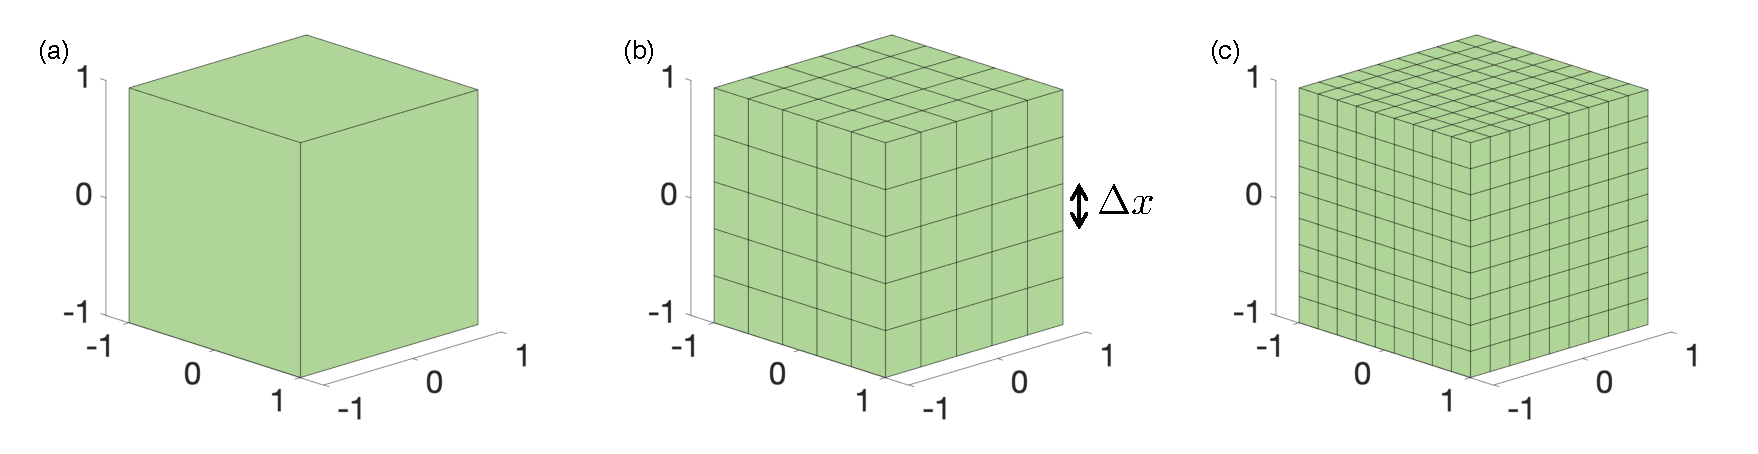
\includegraphics[scale=0.45]{./figures/fig_cube_all_dx}
	\end{center}
	\caption{Cubes of various resolutions used for validation. All three cubes have the same volume and contain (a) 1 interior cube with length $\Delta x = 2$ (b) $5^3=125$  interior cubes with length $\Delta x = 2/5$, and (c) $9^3 = 729$  interior cubes with length $\Delta x = 2/9$.}
	\label{fig_test_cubes}
\end{figure}
We proceed to validate and compare our implementation of the single and double-layer approaches. Although the single-layer approach is somewhat simpler to implement, it has been found to yield linear systems with larger condition numbers when integrated using boundary element methods, though with seemingly little impact on its accuracy \cite{youngren_stokes_1975,ingber_comparison_1999}.
We consider a simple system where resolution may easily be varied and compute the flow around a single large cube, subdivided into smaller collated cubes, as shown in Fig. \ref{fig_test_cubes}.
We define $\Delta x  = 2 / N_x$, where $N_x$ is the number of cubes in each linear dimension, and increase the resolution by increasing $N_x$.
The prescribed translation and angular velocities are kept constant at $\vec{U}'_a = (0,0,-1)$ and $\vec{\Omega}'= (0,0,0)$, respectively. We then compute and compare the total force and torque on the cube. 
\par
\begin{figure}[ht]
	\begin{center}
		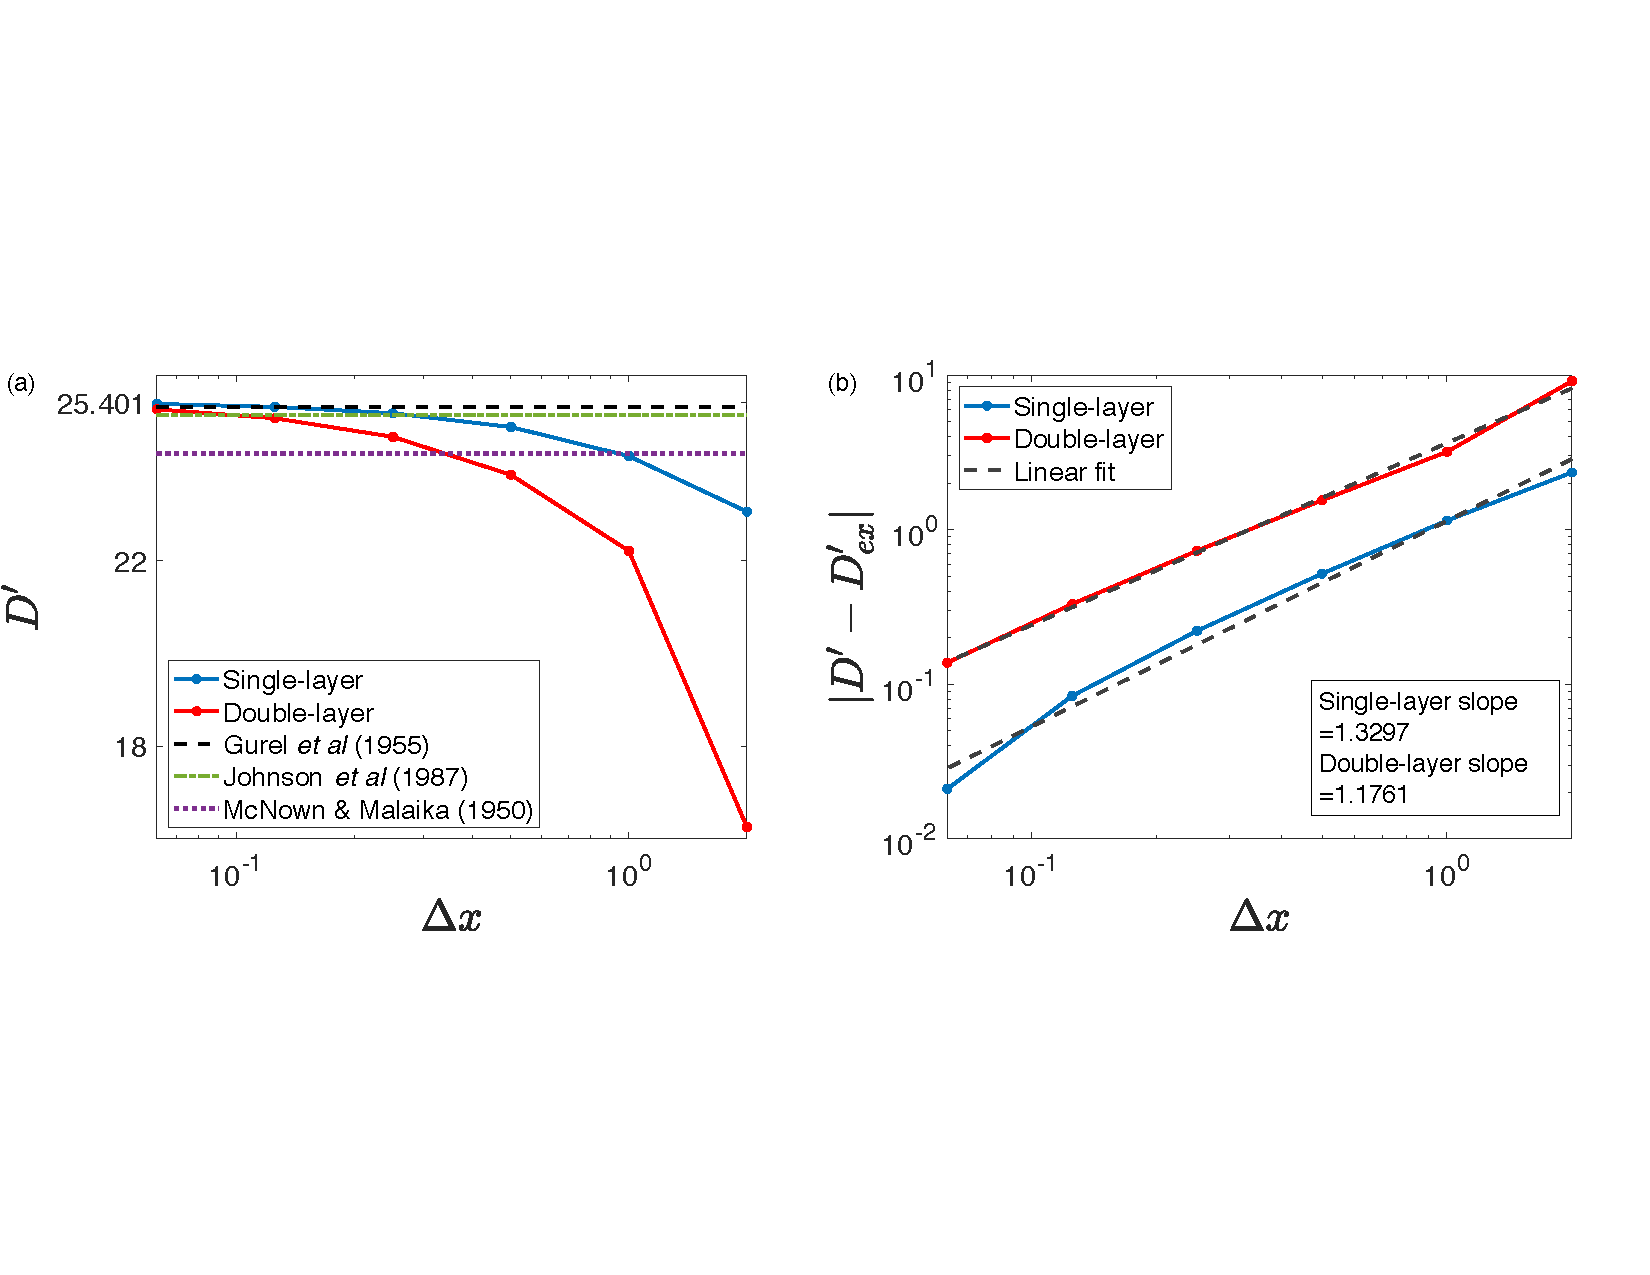
\includegraphics[scale=0.5]{figures/fig_compare_drag_error}
	\end{center}
	\caption{(a) Drag on a cube as a function of $\Delta x$ for both the single- and double-layer methods. (b) Error of the drag as $\Delta x$ is varied, shown on a loglog scale. Dashed lines are linear fits to the data. The error is computed by taking the difference between the limit shown in (a), $D'_{ex} = 25.401$, and drag values, $D'$, when $\Delta x = 2, 1, 0.5,   0.25,  0.125,$ and $0.0625$. }
	\label{fig_drag_compare}
\end{figure}
In  Fig. \ref{fig_drag_compare}(a), we present the non-dimensional drag, $D'$, the $z'$-component of the total force on the cube, 
\begin{equation}
D' = -\vec{F}' \cdot \frac{\vec{U}_a}{||\vec{U}_a||} =  \vec{F}' \cdot \hat{k} =  \frac{\vec{F} \cdot \hat{k}}{ \tilde{\mu} U_s L}, 
\label{eq_drag}
\end{equation}

as computed by both methods, using equations (\ref{eq_forcebal}) and (\ref{alpha_dl_nonD}), for various resolutions. We first observe that both methods converge to the same limit value of $D'  \approx 25.401$ as we decrease $\Delta x$.
These results agree very well with the observations of
Gurel {\textit et al.} 
\cite{gurel_studies_1955} who found a drag of 25.311, and with the empirical relation proposed by 
Johnson {\textit et al.} 
\cite{johnson_drag_1987}, which yields a drag of 25.150. Values given in earlier literature are similar but somewhat smaller, with 
 McNown \& Malaika  \cite{mcnown_effects_1950} 
reporting a drag of 24.311. These literature values are also plotted in  Fig. \ref{fig_drag_compare}(a).
\par
Fig. \ref{fig_drag_compare}(b) presents the error relative to the limit value of $D'_{ex}  = 25.401$ for both methods.
We notice that the convergence rate is similar in both methods, showing a convergence rate slightly higher than one. 
 Typically, one expects to observe a quadratic order of convergence using the mid-point integration rule. However, the order of convergence is likely lower here owing to the presence of edges and corners, which are not treated specially as resolution is increased.
 \par
The single-layer method is seen to be more accurate than the double-layer method, with an error approximately four times smaller. In other words, a similar degree of accuracy can be obtained with the single-layer method when using a value of $\Delta x$ four times greater than the double-layer method.
The other components of the force acting on the cube as well as the total torque are expected to be exactly zero because of the symmetry of the cube.
In our computations, the torque and the other components of the force never exceed $10^{-10}$, as anticipated. 

\begin{figure}[ht]
	\begin{center}
		\epsfig{figure=figures/fig_sample_cube_new, scale=0.11}
	\end{center}
	\caption{The shaded face is the domain where the stress vector and density shown in Fig. \ref{fig_stress_cube8_32} and	\ref{fig_density_cube8_32} are computed. The red arrow shows the $x$-axis used in Fig.  \ref{fig_cross_section}. Sample  streamlines, discussed in Section \ref{ch_streamlines}, are shown as dashed lines. We also show the translation vector,  $\vec{U}'_a$.}
	\label{fig_face_description}
\end{figure}


\begin{figure}[ht]
	\begin{center}
		\epsfig{figure=figures/fig_stress_all, scale=0.5}
	\end{center}
	\caption{Vertical ($z'$) component of the stress vector, $\vec{f}'$, computed using the single-layer potential shown at $z'=1$, as illustrated in Fig. \ref{fig_face_description}. The resolution is: (a) $\Delta x = 2$, (b) $\Delta x = 0.5$, and (c) $\Delta x =  0.0625$. The color bar is the same for all three figures.  }
	\label{fig_stress_cube8_32}
\end{figure}


\begin{figure}[ht]
	\begin{center}
		\epsfig{figure=figures/fig_density_all.pdf, scale=0.5}
	\end{center}
	\caption{Vertical ($z'$) component of the density, $\vec{\psi}'$, computed using the double-layer potential, shown at $z'=1$, as illustrated in Fig. \ref{fig_face_description}. The resolution is: (a) $\Delta x = 2$, (b) $\Delta x = 0.5$, and (c) $\Delta x =  0.0625$. The color bar is the same for all three figures and the same as in Fig. \ref{fig_stress_cube8_32}.}
	\label{fig_density_cube8_32}
\end{figure}
\par
We now consider point-wise quantities such as the stress vector, density function, and velocity on the surface of the cube and in the fluid exterior to the cube. 
These quantities are computed in the plane $z'=1$, which coincides with the face of the cube normal to the incoming flow, as shown in Fig. \ref{fig_face_description}. 
We show in Fig. \ref{fig_stress_cube8_32} and \ref{fig_density_cube8_32} the $z'$-component of the stress vector, $\vec{f}'$, and of the density, $\vec{\psi}'$, 
respectively. 
When varying the resolution of the cube,  we obtain $N_x^2$ different values of the stress vector or density for each side of the cube, each assumed to be constant on a square with side length $\Delta x$.
Comparing Figs. \ref{fig_stress_cube8_32} and \ref{fig_density_cube8_32}, it is clear that the stress vector is better approximated by a constant value than the density.
 As can be seen in both Fig. \ref{fig_stress_cube8_32} and \ref{fig_density_cube8_32}, convergence is slowest at the edges and even more so at the corners. Despite the rapid variations of the stress vector and density at the corners, the drag is seen to converge with increased resolution, see Fig. \ref{fig_drag_compare}, though perhaps with a slower order of convergence than would be expected from a mid-point rule.
 The single-layer potential approach thus provides a good approximation of the total drag even at low resolution. In contrast, the double-layer potential method finds a density that is varying to a greater extent over the face of the higher-resolution cube, making low resolution estimates less accurate. On the other hand, the variations near the corners are smoother, which could make this method a better choice if one were focusing on the behavior at the edges or corners.  These observations are consistent with the single-layer approach resulting in more accurate computations of the drag than the double-layer approach when using the same resolution.
 \par
 \begin{figure}[ht]
	\begin{center}
		\hspace{0.1cm}
		\epsfig{figure=figures/fig_vel1d_all.pdf,scale=0.4}
	\end{center}
	\caption{Vertical ($z'$) component of the velocity, denoted by $w'$, along the line $(x',0,1)$ as illustrated in Fig. \ref{fig_face_description}.  We show three different resolutions for the (a) single-layer method and (b)  double-layer method.}
	\label{fig_cross_section}
\end{figure}

We next present analysis of the $z'-$component of the velocity, $w'$, when the cube has the same translation velocity, $\vec{U}'_a = (0,0,-1)$.
In Fig. \ref{fig_cross_section}, we present this velocity along the line $(x',0,1)$,  shown in Fig. \ref{fig_face_description} as the red arrow, 
as we vary the resolution of the cube for both the single-layer and double-layer approaches.
When using the single-layer potential, we 
compute the velocity for all points using equation (\ref{eq_BI_sl_ND}). For the double-layer potential approach, we 
compute the velocity at points on the surface of the cube using equation (\ref{eq_BI_DL_jump_noD})  and at points in the fluid exterior to the cube using equation  (\ref{eq_BI_DL_noD}).
In Fig. \ref{fig_cross_section}, dashed lines represent the edge of the cube,  i.e. points $x' \in [0,1]$ are on the cube surface and points $x' \in (1,2]$ are exterior to the cube. Since we impose the translation velocity, $\vec{U}'_{a}$ at the center of each square, we expect that $w'= -1$ for $x' \in [0,1]$.
We observe that on the cube surface, the single-layer method, shown in Fig. \ref{fig_cross_section}(a), results in smoother velocities than the double-layer method, shown in  Fig. \ref{fig_cross_section}(b).
In Fig. \ref{fig_cross_section}(a), as $\Delta x$ decreases, the velocities on the surface of the cube are converging to $-1$. The velocity on the edge of the surface, at $x' = 1$, does not agree exactly with the expected value, though it approaches -1  as $\Delta x$ decreases.  On the other hand, the double-layer approach has discontinuous oscillations of the velocity on the surface. This is due to our assumption of locally constant, and thus discontinuous, $\vec{\psi}'$, which directly affects the velocity in equation (\ref{eq_BI_DL_jump_noD}).  The oscillations decrease in amplitude as $\Delta x$ decreases, and the velocity exterior to the cube is smooth. The discrepancy with the expected velocity at the edge of the cube, $x' =1$, is greater than for the single-layer approach.

\begin{figure}[ht]
	\begin{center}
		\hspace{0.1cm}
		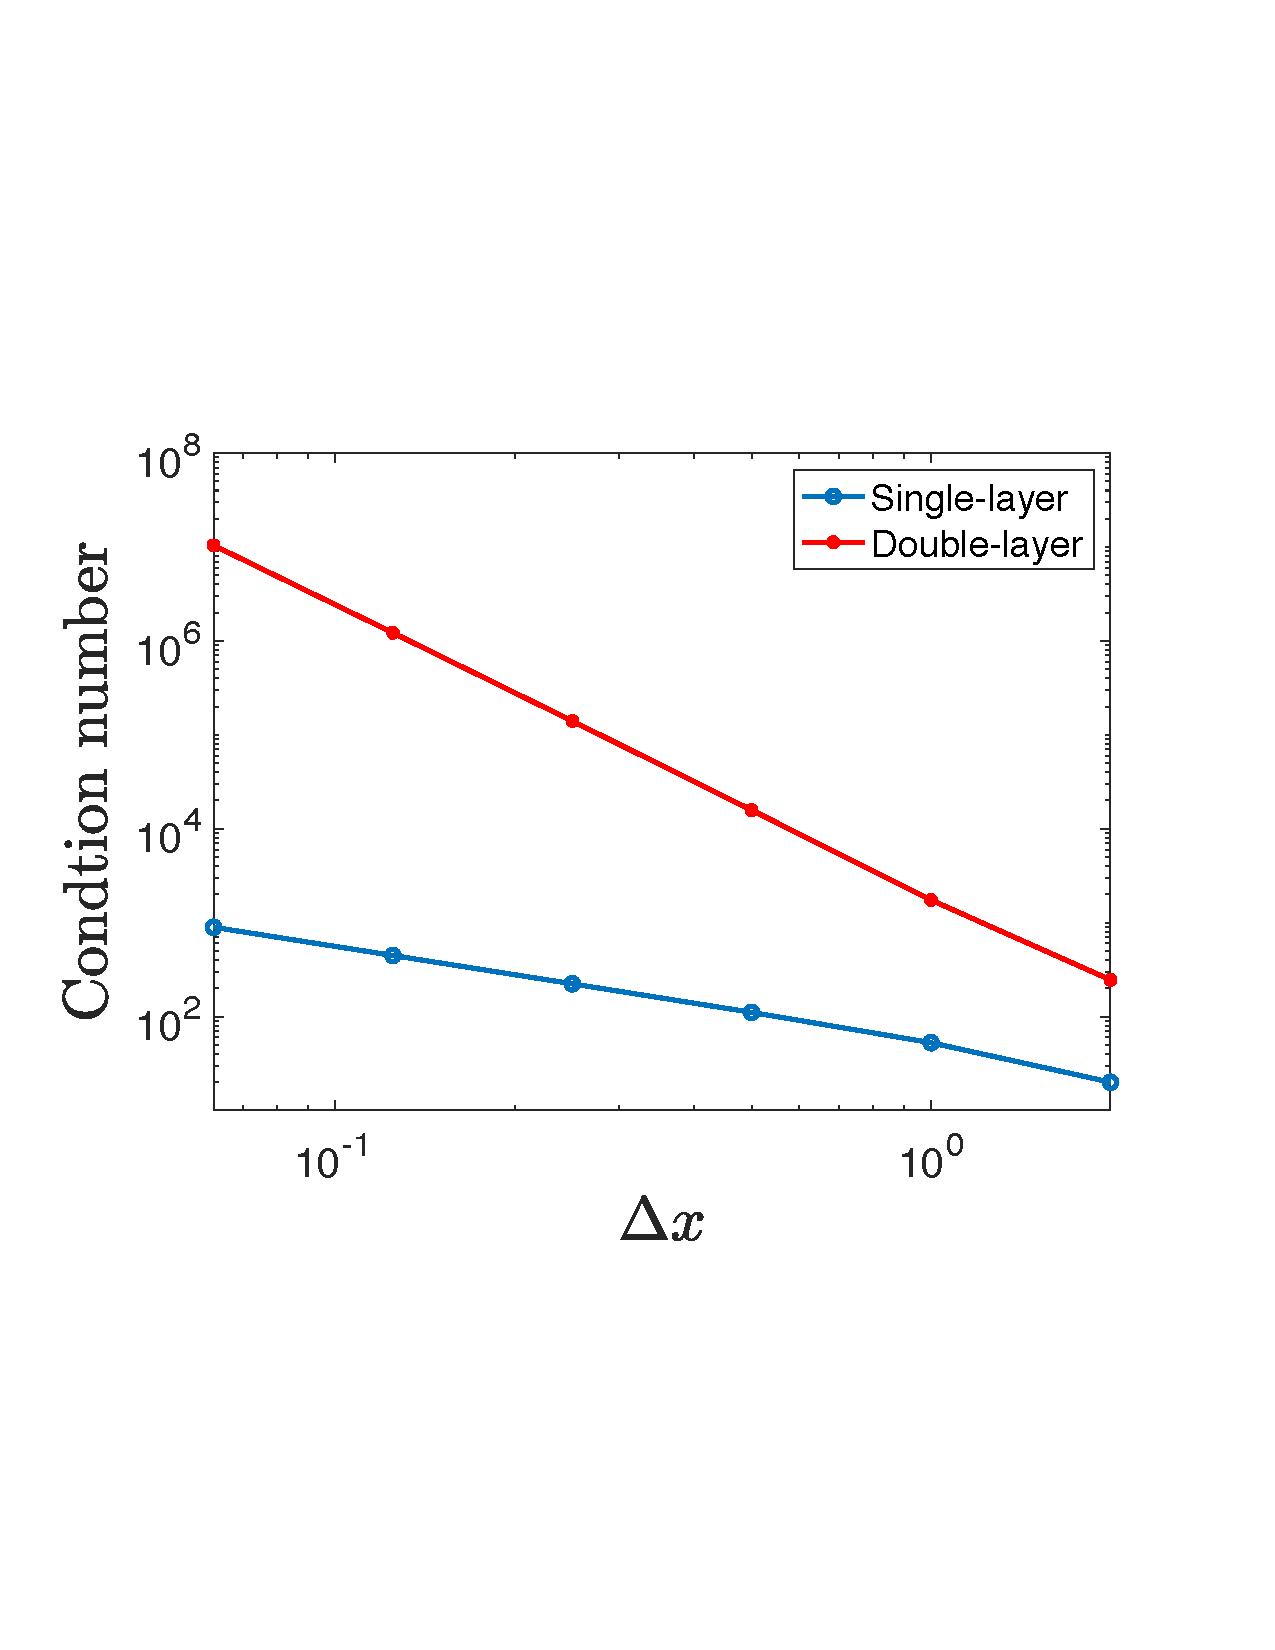
\includegraphics[scale = 0.5]{./figures/fig_con_new}
	\end{center}
	\caption{Comparison of the condition number for the linear system of both the single-layer and double-layer methods as the resolution of the cube is varied. }
	\label{fig_condition_number}
\end{figure}
\par
We conclude the comparison of the two methods by considering their computational complexity.
It has been observed that Fredholm integral equations of the  first kind, such as that associated with the single-layer potential, often lead to ill-posed numerical
methods when the surface integral is discretized \cite{delves_numerical_1974, karrila_integral_1989}.
The main challenge is dealing with the singularity of the 
the integral kernel. However, in our method, we compute the surface integrals analytically over each square, so that the kernel singularities are integrated exactly. In addition, we constrain the system to have a unique solution through equation (\ref{eq_constraint}). We compare the condition number of the linear system of each of our two methods for various resolutions in Fig. \ref{fig_condition_number}. We find that the condition number
of the single-layer method is approximately inversely proportional to $\Delta x$. 
On the other hand, the condition number of the double-layer method is approximately inversely proportional to $(\Delta x)^{3}$, and is thus much greater.
\par
Based on our findings of more accurate drag, smoother and more accurate velocity, and smaller condition number,  we conclude that the single-layer potential approach is more appropriate to model flow around aggregates made of cubic particles. 
In the remainder of this paper, we therefore present results obtained using the single-layer approach.
%-----------------
\subsection{Streamlines} 
\label{ch_streamlines}
To gain a better understanding of the flow around a cube, we present the streamlines generated when $\vec{U}'_a = (0,0,-1)$. We show the streamlines around the cube in the frame of reference of the cube for $y' = 0$ in Fig.  \ref{fig_strlns} 
(see Fig. \ref{fig_face_description} for the exact location of the face and sample streamlines).
To compute the streamlines, we first obtain the values of stress vector, $\vec{f}'(\vec{x}'_s)$, on each square face of the cube using equation (\ref{eq_BI_sl_ND}).
We then chose initial positions below the cube and use a second order Runge-Kutta method to advance the positions in time using the corresponding velocities computed using equation (\ref{eq_BI_sl_ND}) at each position. 
We compare the streamlines with four different resolutions of the cube; $\Delta x = 2,1, 0.5,$ and $0.25$. For the cube with $\Delta x = 2$, streamlines are seen to enter the interior of the cube. As we increase the resolution, the streamlines remain exterior to the cube.
Moreover, higher resolutions result in streamlines following the cube  boundary more accurately, showing the convergence of the method.
\begin{figure}[ht]
	\begin{center}
		\epsfig{figure=figures/fig_strlns_horizontal-compressed.pdf, width=150mm}
	\end{center}
	\caption{Streamlines around a cube with varying resolution moving in the $z'-$direction. The resolution is: (a) $\Delta x = 2$, (b) $\Delta x = 1$, (c) $\Delta x  =0.5$, and (d) $ \Delta x =0.25$. }
	\label{fig_strlns}
\end{figure}
%-------------------------------------
\section{Results: Forces on Aggregates Subject to a Background Flow} 
\label{sec:results}
In this section, we present the response of aggregates when subjected to various flow fields. We consider an aggregate at rest, with boundary condition $\vec{u}'=0$ on the surface of the aggregate, subject to a background flow. Three common background flows are considered, which can be combined to provide an approximation of any general flow to first order in space: $\vec{U}'_{bg}(\vec{x}) = -\vec{U}'_a - \vec{\Omega}' \times \vec{x}' + \bar{\bar{M}}' \cdot \vec{x}'$, the primes indicating dimensionless quantities as above. Here, $-\vec{U}'_a$ is the translation velocity of the flow past an aggregate or equivalently when changing frame of reference, a constant settling velocity $\vec{U}'_a$ of the aggregate in a fluid at rest.  Similarly, $-\vec{\Omega}'$ is the constant angular velocity of a rotating flow around an aggregate, or equivalently when changing frame of reference, the constant angular velocity of a rotating aggregate in a fluid at rest. Lastly, $\bar{\bar{M}}'$ is a traceless, symmetric tensor that induces a straining flow around the aggregate. In all three cases, to solve for the response of the aggregates, we decompose the fluid velocity as $\vec{u}' = \vec{U}'_{bg} + \vec{U}'_c$, where the correction velocity, $\vec{U}'_c$, decays to zero at infinity and satisfies $\vec{U}'_c = -\vec{U}'_{bg}$ on the surface of the aggregate. 
Using this formulation allows for this correction to be computed via the single-layer potential boundary integral as described above in Sections \ref{section3} and \ref{sec:numerical}.
\subsection{Translation Flow}
\label{sec:results_translationflow}

\begin{figure}[ht]
	\begin{center}
		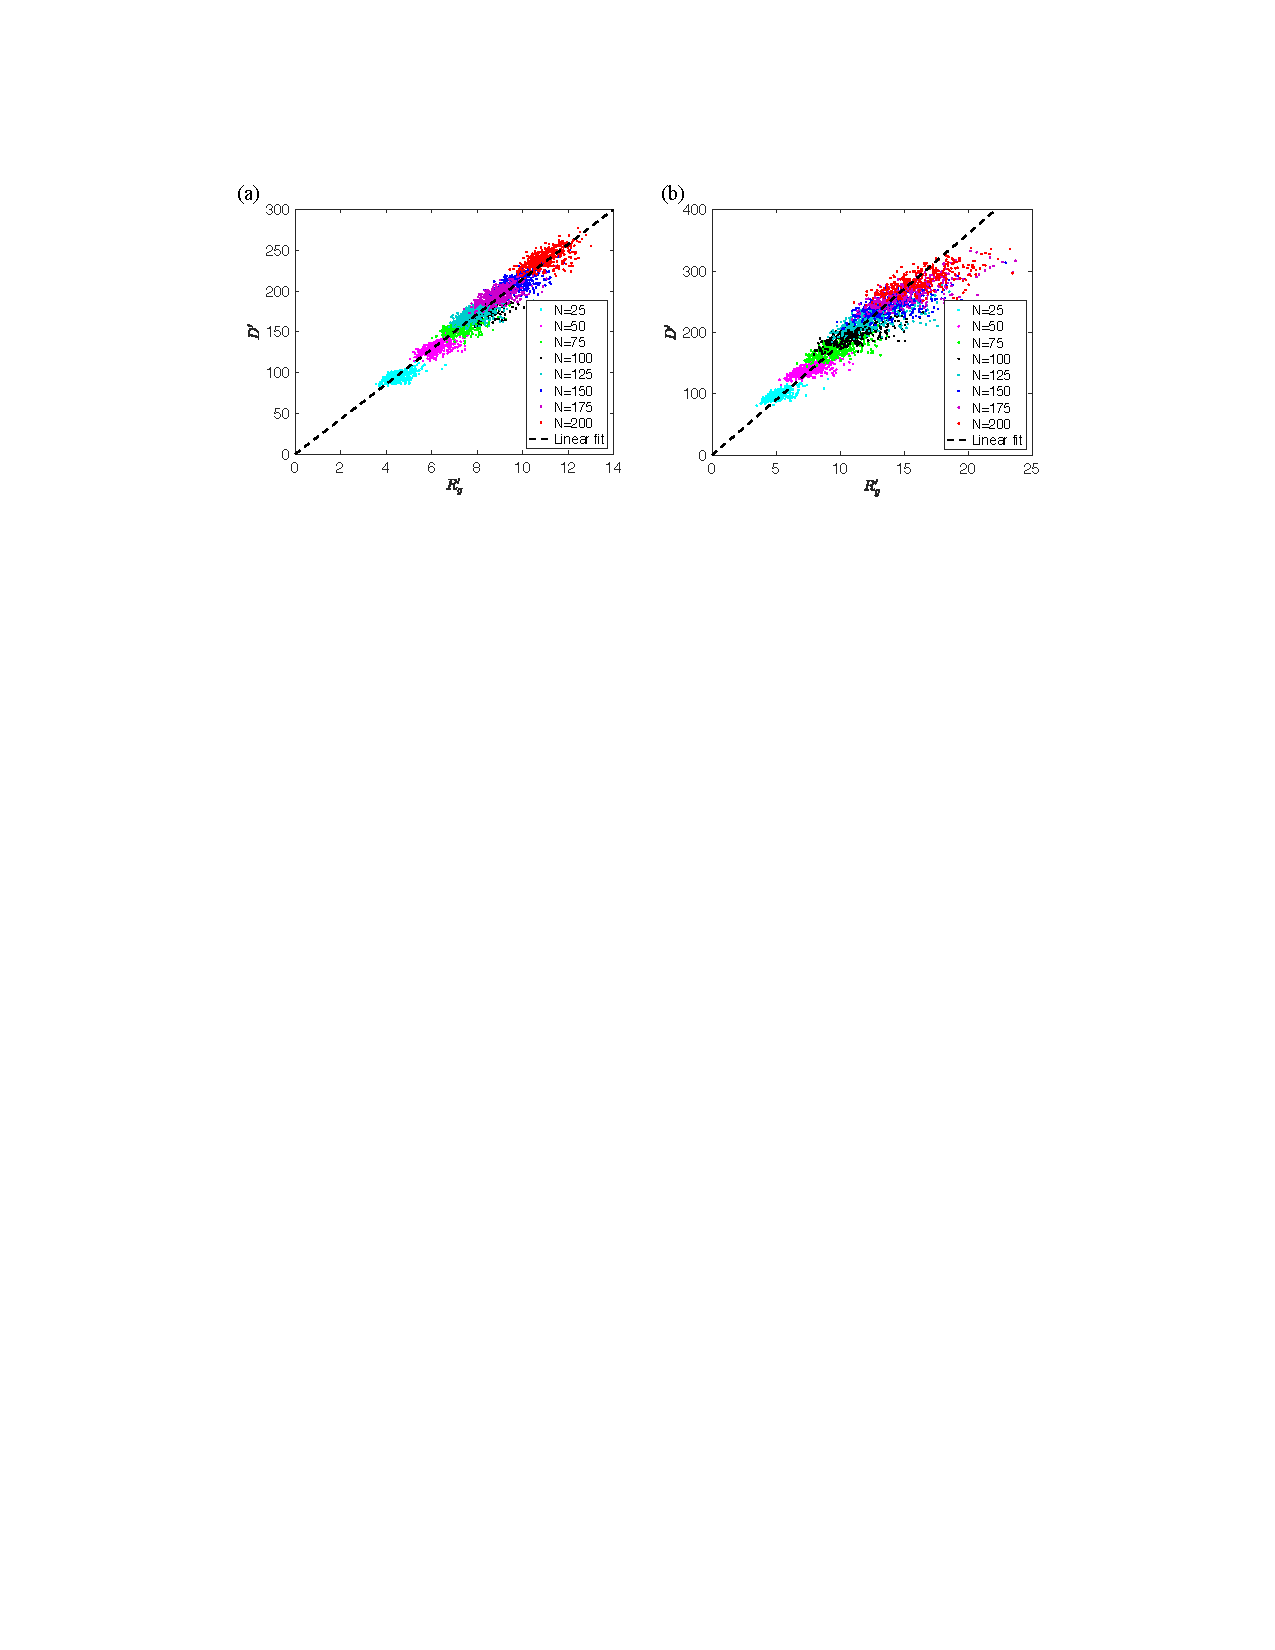
\includegraphics[scale = 1.0]{./figures/fig_drag_allprime.pdf}
	\end{center}
	\caption{Non-dimensional drag of aggregates in a constant flow, $\vec{U}'_{bg} = -\vec{U}'_a = (0,0,1)$, as a function of gyration radius $R'_g$ for aggregates of different sizes, $N$. We present in (a) the drag of individually-added-aggregates (IAA) and in (b) the drag of cluster-cluster-aggregates (CCA). The dashed lines are least-square linear fits: in (a) $D' = 21.47 R'_g$ and in (b) $D' =18.04 R'_g$.}
	\label{fig_drag_raw}
\end{figure}

We first consider a constant background velocity, $\vec{U}'_{bg}(\vec{x}') = -\vec{U}'_a=(0,0,1)$. In Fig. \ref{fig_drag_raw} we present the non-dimensional drag on the aggregate, $D'$, as defined in equation (\ref{eq_drag}),
 as a function of the non-dimensional gyration radius, $R'_g$, of each aggregate. We show in Fig. \ref{fig_drag_raw}(a) the drag on aggregates formed by individual random walkers (IAA), and in Fig. \ref{fig_drag_raw}(b) the drag on aggregates formed by cluster aggregation (CCA).
 Recall that  aggregates formed by individually-added random walkers tend to be more compact.
The drag appears to scale linearly with the gyration radius for both types of aggregates, as would be expected from dimensional considerations for the proper measure of the size of an aggregate. 
Note that for all the fits presented in this section, we compute the coefficient of determination, $\mathbf{R}^2$, using either the gyration or maximum radius as an independent variable, to assess how closely each model fits the data. 

To verify this linear relationship between the drag and the gyration radius, we found the slope of $D'$ as a function of $R'_g$ on a loglog plot, giving the best exponent, $\alpha$, in the relation $D' \sim (R_g')^\alpha$. This confirmed that a linear fit was optimal for IAA, finding $\alpha=1.00$, and found a somewhat smaller exponent for CCA, with $\alpha=0.85$. Assuming a linear relation, we find
for individual aggregation (IAA) that a least-square fit has a slope of 21.47 with  a coefficient of determination of $\mathbf{R}^2=0.95$ (Fig. \ref{fig_drag_raw}(a)) 
For cluster aggregation (CCA), we find a best-fit line with slope 18.04, and a corresponding coefficient of determination of $\mathbf{R}^2=0.86$ (Fig. \ref{fig_drag_raw}(b)). 



These results are consistent with experimental results which showed a linear relationship between the drag on an aggregate and the square root of $A^\prime_p$, the two-dimensional projected area of the aggregate \cite{tang_model_2002}.  In addition to computing the drag as a function of the gyration radius, we computed the drag of aggregates as a function of their projected area. We found that $A^\prime_p$ was not as good predictor of the drag experienced by the aggregate. In particular, for aggregates containing a fixed number of cubes, we observed no correlation between the projected area and the drag experienced by the aggregate. A similar observation holds for the torque and straining force discussed below, and as a result, we choose to present all of our results in terms of either the maximum or gyration radius.

\begin{figure}[ht]
	\begin{center}
		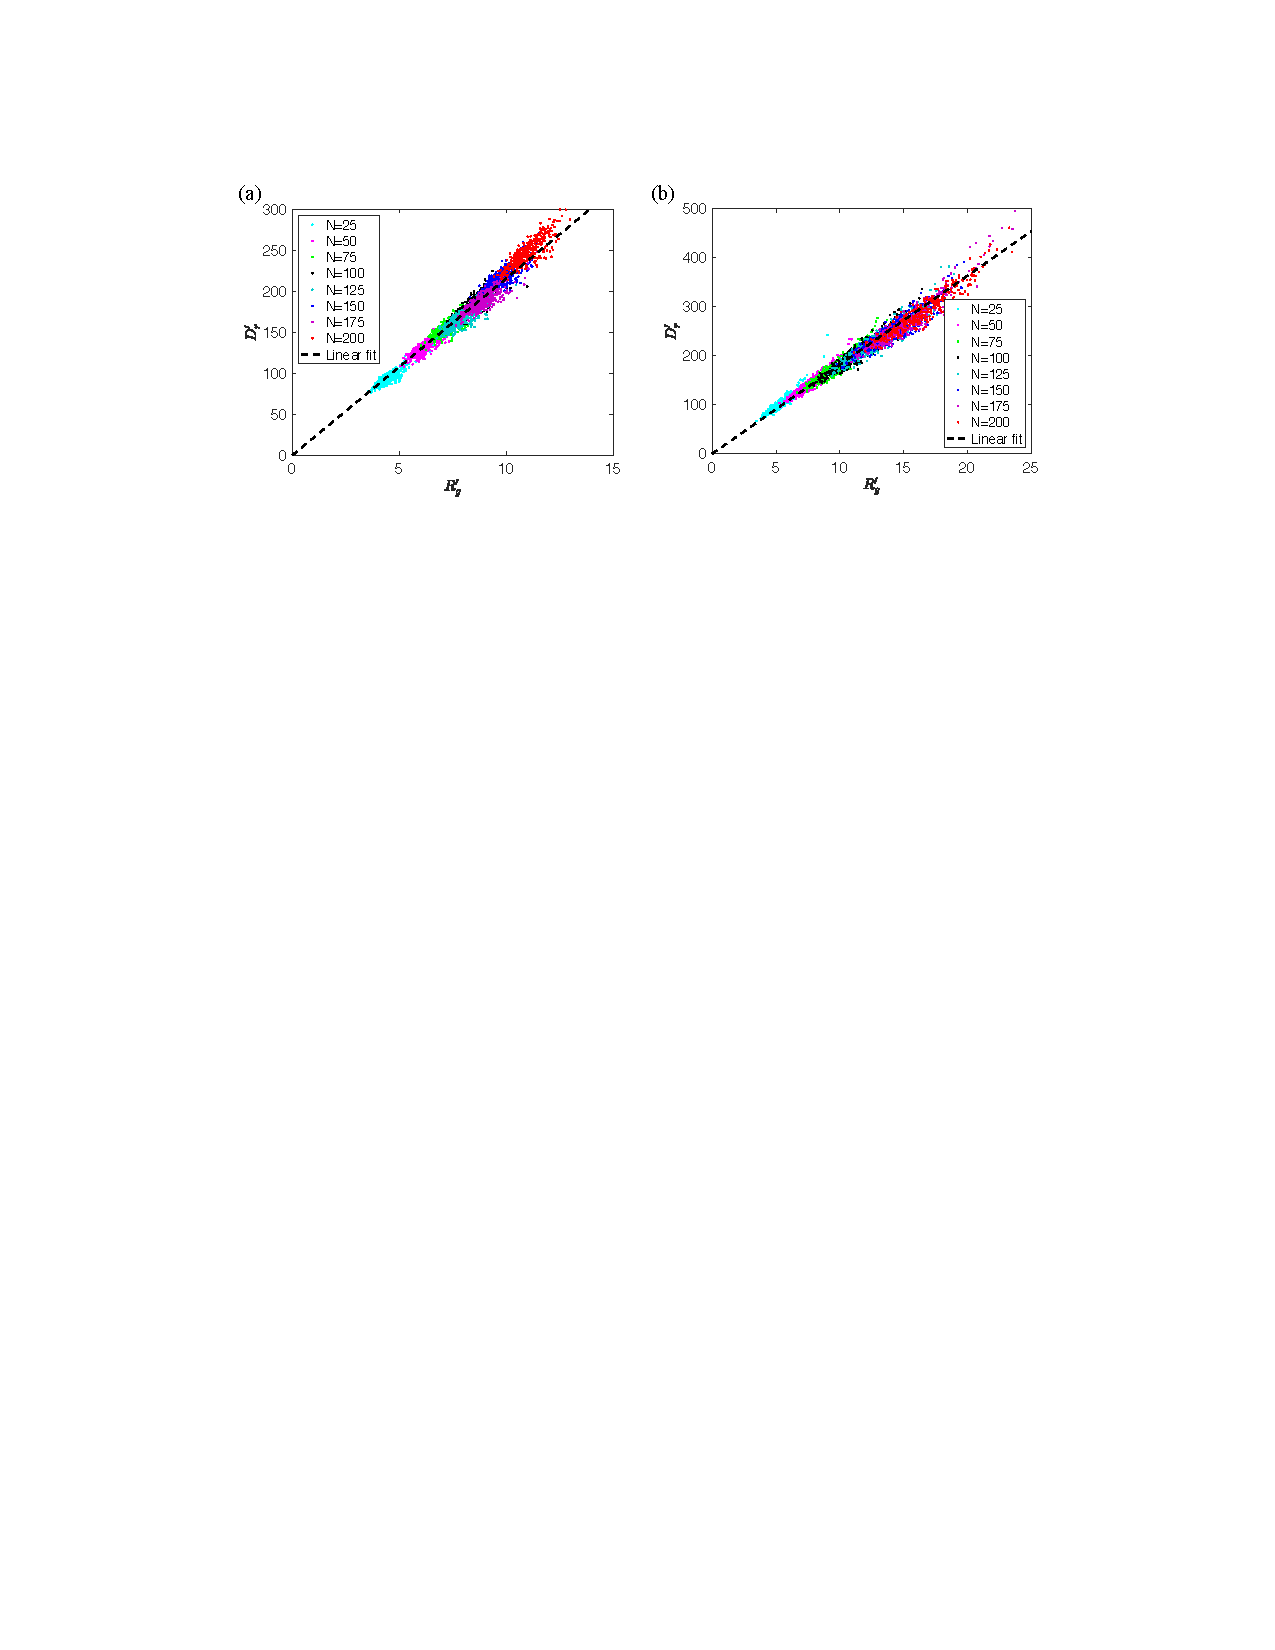
\includegraphics[scale = 1.0]{./figures/fig_drag_all_rescaledprime.pdf}
	\end{center}
	\caption{Rescaled non-dimensional drag, $D'_r$, as a function of gyration radius $R'_g$ for (a) individually-added aggregates (IAA) and for (b)  
	cluster-cluster-aggregates (CCA). The rescaled drag, $D'_r$, is defined in equation (\ref{def_drag_rescaled})  and the fits to the data, plotted as dashed lines, are given in equation (\ref{eq_drag_rescaledIAA}) for (a) and in equation (\ref{eq_drag_rescaledCCA}) for (b).}
	\label{fig_drag_rescaled}
\end{figure}

Although the relationship between the drag and gyration radius is nearly linear, there appears to be further structure in the data obtained, as is particularly visible for CCA in Fig. \ref{fig_drag_raw}(b). For an aggregate composed of a fixed number of cubes, $N$, the drag increases linearly with aggregate size, but at a slower rate than when $N$ is also allowed to vary. To better characterize this dependency, we introduce a rescaled non-dimensional drag that takes into account the difference between the gyration radius of a given aggregate and the mean gyration radius of all aggregates with the same number of cubes.
We denote the average gyration radius for aggregates of $N$ cubes as $\bar{R}'_g(N)$. Similarly, 
we define an average maximum radius for aggregates made of $N$ cubes as $\bar{R}'_m(N)$. We may then define the departure from these average value as 
\[
\sigma_g = \frac{R'_g - \bar{R}'_g}{\bar{R}'_g} \text{\ \ \ \ \ \ and \ \ \ \ \ \ } \sigma_m = \frac{R'_m - \bar{R}'_m}{\bar{R}'_m}.
\]
These measures are positive when the aggregate is more spread out than the mean aggregate size and negative when the aggregate is more compact than the mean. We use these measures to define a rescaled drag that accounts for the variability in the aggregate radius as 
\begin{equation}
D'_r = \frac{D'}{1 + \gamma \sigma_g} \, , 
\label{def_drag_rescaled}
\end{equation}
where $\gamma$ is an empirical parameter that we fit based on the data. To optimize the collapse, we choose $\gamma$ to maximize the correlation coefficient between the rescaled drag and the gyration radius.  


As seen in Fig. \ref{fig_drag_rescaled} the data collapses better. For IAA, we find $\gamma = -0.43$, with a best-fit line of  $D_r' = 21.55 R'_g$, which improves the coefficient of determination to 0.97, which is a relatively small gain as the data was already nearly linear. This negative value of $\gamma$ indicates that less compact aggregates experience more drag than more compact aggregates when composed of the same number of cubes.
The drag is thus well described by
\begin{equation}
D' = 21.55 \left(1 - 0.43  \frac{R'_g - \bar{R}'_g}{\bar{R}'_g}\right )  R'_g \, . 
\label{eq_drag_rescaledIAA}
\end{equation}
where the mean gyration radius is $\bar{R}'_g = 1.32N^{0.39}$, as described in Section 3.
For CCA,  the same procedure yielded $\gamma = -0.64$, and the resulting collapse is shown in Fig. \ref{fig_drag_rescaled}(b).
The rescaled drag follows a much improved linear relationship as a function of the gyration radius, with a slope of 18.16 and a coefficient of determination of $\mathbf{R}^2=0.97$. A complete description of the drag for CCA is thus
\begin{equation}
D' = 18.16 \left(1 -0.64  \frac{R'_g - \bar{R}'_g}{\bar{R}'_g}\right) R'_g
\label{eq_drag_rescaledCCA}
\end{equation}
where the mean gyration radius is $\bar{R}'_g = 0.85N^{0.56}$.  
A similar dependence was found when replacing the gyration radius with the maximum radius or the square root of the projected area. However, the coefficients of determination were then lower, by approximately 2\%, and the best fit exponents, $\alpha$, were lower for the gyration radius and further from one for the projected area (lower for IAA, higher for CCA). This indicates that the gyration radius is a better descriptor of the size of an aggregate when considering the drag.

\subsection{Rotating flow}

\begin{figure}[ht]
	\begin{center}
	\epsfig{figure=./figures/fig_torque_all.pdf,scale=1}
	\end{center}
	\caption{Non-dimensional torque, $T'$, defined in equation (\ref{eq_Qprime}), as a function of gyration radius, $R'_g$, for aggregates composed of a varying number of cubes, $N$. In (a)  individually-added-aggregates (IAA) are presented and in (b) cluster-cluster-aggregates (CCA) are presented.	The dashed lines are least-square cubic fits: in (a) $T' = 44.12 (R_g')^3$ and in (b) $T' = 24.98 (R_g')^3$.}
	\label{fig_torque}
\end{figure}
In Fig. \ref{fig_torque}, we present the non-dimensional torque as a function of gyration radius for aggregates subject to a rotating background flow, $\vec{U}'_{bg}(\vec{x}') = -\vec{\Omega}' \times \vec{x}'$. We present only the component of the torque parallel to $\vec{\Omega}'$, as the other two components both average to zero. This component, $T'$, is non-dimensionalized using the angular velocity, 
\begin{equation}
T' = -\vec{Q}' \cdot \frac{\vec{\Omega}'}{||\vec{\Omega}' ||}  \text{\ \ \ and \ \ \ } \vec{Q}' = \frac{  \vec{Q} } {\tilde{\mu} ||\vec{\Omega}  || L^3 } 
\label{eq_Qprime}
\end{equation}


Here, we expect a cubic dependence of the torque on a properly chosen measure of the size of the aggregate, 
 in contrast to the linear dependence of the drag as described in Section 
\ref{sec:results_translationflow}. 
This is because computing a torque rather than a force increases the order of dependence on the gyration radius by one. In addition, this calculation is  based on an imposed angular velocity, $\vec{\Omega}'$, rather than a translation velocity, which also increases the order of the dependence on the gyration radius by one.
We verified that a cubic fit was the most appropriate by finding the slope on a loglog plot of the torque as a function of gyration radius, yielding  the best exponent $\alpha$ in the relation $T' \sim (R_g')^\alpha$. This confirmed that a cubic fit was optimal for IAA, with $\alpha=3.00$, and again we observed a somewhat smaller exponent for CCA, with $\alpha=2.68$, indicating that the torque of CCA shows a slower average growth.  Furthermore, for CCA, as can be seen in Fig. \ref{fig_torque}(b), there is noticeably more variability.
Assuming a cubic fit, we find for the IAA a least-square fit of $T' = 44.12 (R'_g)^3$ with coefficient of determination $\mathbf{R}^2=0.91$ and for the CCA a least-square fit of $T' = 24.98 (R'_g)^3$ with coefficient of determination $\mathbf{R}^2=0.81$. Here too, a similar dependence was found when replacing the gyration radius with the maximum radius or projected area, though again with smaller coefficients of determination and best fit exponents further from three as expected from dimensional analysis, so that the gyration radius is also more useful descriptor of the size of an aggregate when studying the torque.


\subsection{Extensional flow}


\begin{figure}[ht]
	\begin{center}
		 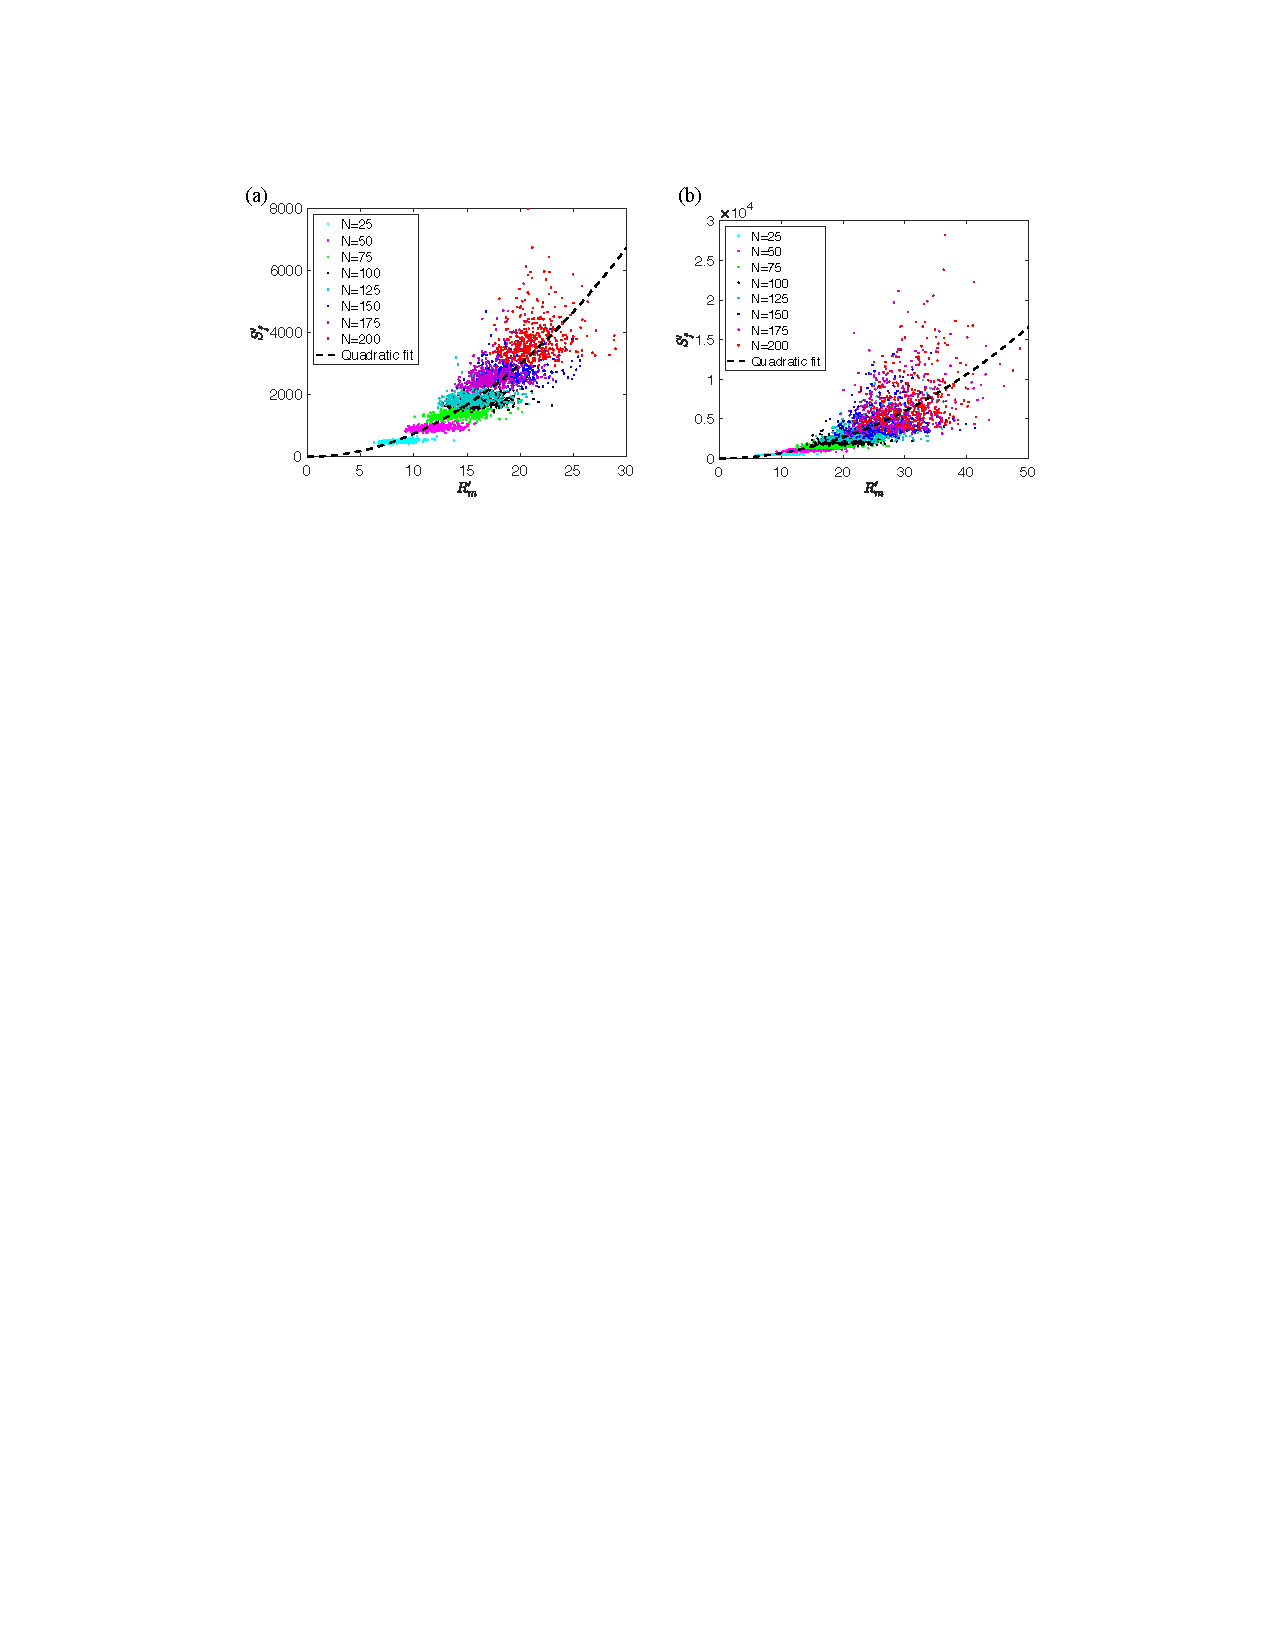
\includegraphics[scale = 1.0]{./figures/fig_strain_allprime.pdf}
	\end{center}
	\caption{Non-dimensional straining force, $S_f'$, defined using equations (\ref{eq_Sf1}) and (\ref{eq_Sf2}), as a function of the maximum radius, $R'_m$, for aggregates of different sizes $N$. In (a) individually-added-aggregates (IAA) and in (b) cluster-cluster-aggregates (CCA) are presented. The dashed lines are least-square quadratic fits: in (a) for IAA, $S_f' =7.48 (R'_m)^2 $ and in (b) for CCA, $S_f'  = 6.64 (R'_m)^2$.}
	\label{fig_strain_maxR}
\end{figure}

We now consider the response of an aggregate to  an extensional flow, $\vec{U}'_{bg}(\vec{x}') = \bar{\bar{M}}' \cdot \vec{x}'$. In such a background flow, for an object with no preferred orientation, the drag and torque both average to zero. However, the aggregate will be under effective tension or compression, an effect that could lead to rupture. Quantifying these forces is relevant to the formation and breakup of marine aggregates. 
We therefore define a straining force vector, $\vec{E}$, that quantifies this effect. 
We non-dimensionalize this force using the largest eigenvalue in magnitude of the matrix $\bar{\bar{M}}$ which we denote by $|\lambda|$, and obtain  
\begin{equation}
\vec{E}' = \frac{\vec{E}}{\tilde{\mu} |\lambda| L^2}.
\label{eq_Sf1}
\end{equation}
The straining force may be decomposed as 
$\vec{E}' = E'_{1} \hat{v}_1 + E'_{2} \hat{v}_2 + E'_{3} \hat{v}_3$, where the $\hat{v}_i$ are the real, orthonormal eigenvectors in the spectral decomposition of $\bar{\bar{M}}'$, which is always possible since $\bar{\bar{M}}'$ is symmetric. 
The components of $\vec{E}'$ are  then defined as
\begin{equation}
E_i' = \frac{1}{2} \left( \int_{S'} | \vec{f}' \cdot \hat{v}_i | \ dS' - \left| \int_{S'} \vec{f}' \ dS' \right|  \cdot \hat{v}_i \right), 
\label{eq_Sf2}
\end{equation}
where $\vec{f}' \cdot \hat{v}_i$ is the projection of the stress vector in the direction of the eigenvector $\hat{v}_i$. 
This straining force is a measure of how much stress imposed in one direction is also applied in the opposite direction resulting in a strain on the aggregate. The factor of $1/2$ accounts for the double counting of the tensile or compressive forces when integrating the stress vector in the direction of, and opposite to, the vector $\hat{v}_i$. We have subtracted the component of the net force in each direction to obtain a straining force that is independent of the net force on the object. In the results shown in this section, we consider two-dimensional extensional flows, for which the eigenvalues are $-1$ in the $x'$-direction, $1$ in the $y'$-direction, and  0 in the $z'$-direction. We present the component of the straining force in the $y'$-direction, denoted as $S_f'$.

For the straining force, dimensional considerations lead us to expect a quadratic dependence on an appropriate measure of the aggregate's size. However, we found  that the slope of the straining force as a function of gyration radius on a loglog plot, giving the exponent $\alpha$ in the relation $S'_f \sim (R_g)'^{\alpha}$, yielded values greater than two for both IAA and CCA, with exponents of 2.1 and 2.2, respectively. In contrast, using the maximum radius as a measure of the aggregate's size resulted in a dependence that was much closer to being quadratic, with best fits on the growth exponent giving $S_f' \sim (R'_m)^{1.98}$ for IAA and $S_f' \sim (R'_m)^{2.01}$ for CCA. 
We therefore present the data as a function of the maximum radius rather than the gyration radius, as $R'_m$ appears to be a better predictor of the straining force.
In Fig. \ref{fig_strain_maxR}, we present $S_f'$ for aggregates 
of different sizes as a function of the maximum 
radius, $R'_m$. 
The dashed lines in  Fig. \ref{fig_strain_maxR}  are quadratic fits to the data as a function of maximum radius and we find best fits of $S_f' = 7.48 (R'_m)^2$ for IAA with the coefficient of determination of $\mathbf{R}^2=0.74$, and $S_f' = 6.64 (R'_m)^2$ with the coefficient of determination of $\mathbf{R}^2=0.56$ for CCA. For both IAA and CCA, we observe that if $N$ is held constant and the maximum radius is varied, the growth of the straining force seems to be significantly slower than quadratic. This once again suggests a rescaling as in Section \ref{sec:results_translationflow}. 

\begin{figure}[ht]
	\begin{center}
		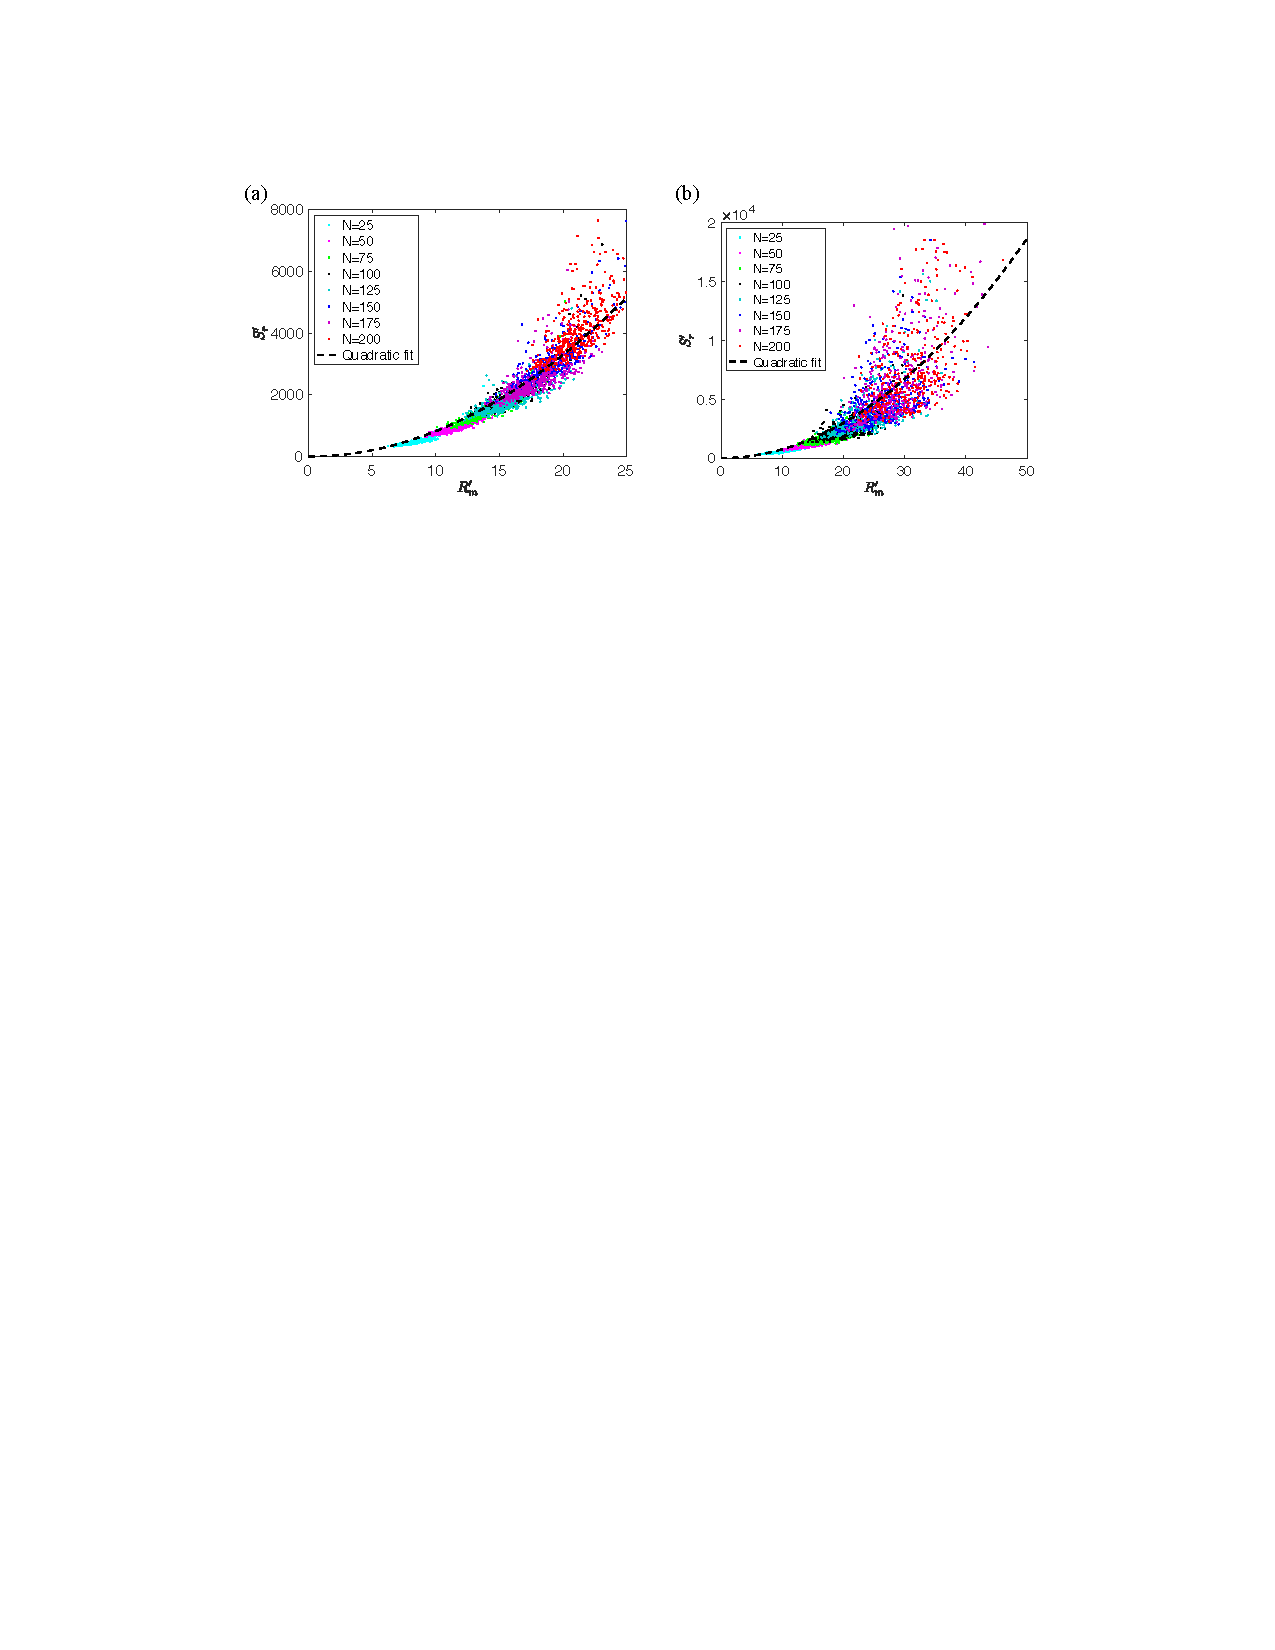
\includegraphics[scale = 1.0]{./figures/fig_strain_all_rescaledprime.pdf}
	\end{center}
	\caption{Rescaled non-dimensional straining force, $S'_r$, as a function of maximum radius $R'_m$ for aggregates of different sizes $N$. In (a) individually-added-aggregates (IAA) and in (b) cluster-cluster-aggregates (CCA) are presented. The dashed lines are least-square quadratic fits: in (a) for IAA, $S'_r = 8.24  (R'_m)^2 $, in (b) for CCA, $S'_r = 7.47 (R'_m)^2 $. }
	\label{fig_strain_maxR_rescaled}
\end{figure}


To rescale the straining force, we define
\[
S'_r = \frac{S'_f}{1 + \gamma \sigma_m},
\label{eq_strain_rescaled}
\]
with $\sigma_m$ defined above as the non-dimensional deviation from the average maximum radius for aggregates of the same size.
This rescaled force yields a better collapse of the data, as can be seen in Fig. \ref{fig_strain_maxR_rescaled}, particularly for IAA. We found that the best rescaling value was $\gamma = -1.32$ for  IAA and $\gamma= -0.92$ for  CCA.  In the CCA case, the resulting data appears to grow slightly faster than quadratic. Nonetheless, it is possible to fit a quadratic to the rescaled drag, and doing so yields $S'_r = 8.24 R_m^2 $ with coefficient of determination $\mathbf{R}^2=0.89$ for IAA and $S'_r = 7.47 R_m^2 $ with coefficient of determination $\mathbf{R}^2=0.63$ for CCA. 


We note that the straining force, even when rescaled, exhibits a large amount of scatter compared to the torque and drag, particularly for CCA, which tend to have more elongated aggregates. Observing individual aggregates of similar size but different straining forces reveals that the straining force is particularly sensitive to the orientation of an aggregate. The scatter is thus largely due to this sensitivity, as the same aggregate oriented differently can experience a significantly different straining force.

%-------Discussion-------------------------------------
\section{Discussion}
\label{sec:discussion} 

The results presented above all use a resolution of $\Delta x=2$, which corresponds to using aggregates made of cubes of non-dimensional side length 2, not further refined. To assess the accuracy of results with this resolution, we considered 16 different aggregates made of 100 cubes of side length two and refined the resolution to use $\Delta x = 2, 1$, and $2/3$, thus increasing the number of cubes from 100 to 800 and 2700 while maintaining the aggregate shape.  
Both the drag and torque were seen to converge as the resolution was increased. The coarsest resolution, used in the section above, yielded results that were less than 2\% away from the more highly resolved results for the drag and less than 5\% away for the torque (we found for similar sampling that the extensional force behaved in a manner between that of the drag and torque).  For comparison, the standard deviation of the drag and torque of the samples considered was approximately three times as large for all resolutions studied. The variability between aggregates of a given size thus far exceeds the error due to a coarse resolution. Further, we performed a similar study on aggregates of various sizes and found that the effects of a coarse resolution decreased as the size of the aggregate increased. 
The data we present is for aggregates of size ranging from 25 to 200 cubes with $\Delta x=2$ and is, therefore, sufficiently accurate to allow a meaningful quantification of the drag, extensional force, and torque. 

To put the results for aggregates obtained in section \ref{sec:results} into context, we compare them to the well-known corresponding results for a sphere \cite{guazzelli_physical_2011}. 
The gyration radius of a sphere of radius $R_s$ is $R_g = \sqrt{2/5} R_s$, and thus the Stokes hydrodynamic force acting on a sphere is $\vec{F} = 6 \pi \tilde{\mu} \vec{U}_a R_s \approx 29.8 \tilde{\mu} \vec{U}_a  R_g$.  Also, the torque on a rotating sphere is $\vec{Q} = 8 \pi \tilde{\mu} \vec{\Omega} R_s^3 \approx 99.35 \tilde{\mu} \vec{\Omega} R_g^3$. For a sphere in an extensional flow, the exact solution of the straining force for the flow satisfying $\vec{U}_{bg} = \bar{\bar{M}}\cdot \vec{x}$ at infinity and $\vec{U}_{bg} = 0$ on the surface of the sphere is known \cite{guazzelli_physical_2011}. The details of the computation of the corresponding straining force are given in the appendix. We find that for a matrix $\bar{\bar{M}}$ with unit eigenvector $\hat{v}_i$ and corresponding eigenvalue $\lambda_i$, the straining force is
\[
E_{i}  = \frac{1}{2} \int_S | \vec{f} \cdot \hat{v}_i | \ dS = 5  \pi \tilde{\mu} R_s^2 \lambda_i \approx 15.7  \tilde{\mu} R_m^2  \lambda_i,
\] 
where we used that the maximum radius $R_m$ of a sphere is simply its usual radius $R_s$ and that a sphere in an extensional flow experiences no net force. 


Our results from Section \ref{sec:results}, and the corresponding results for a sphere, are summarized in Table  \ref{table_sum}. We first note that the hydrodynamic force acting on translating aggregates is significantly less than that acting on a translating sphere of the same gyration radius. This is presumably because the aggregates are not densely filled and thus allow some flow to effectively go through them. For the same reason, the force on the more compact IAA is also greater than that on the less compact CCA.
Similarly, the coefficients of the torque for both types of rotating aggregates are less than those of the corresponding rotating sphere. This is, once again, because less compact structures encounter less torque from the fluid when rotating. Further, a similar observation also holds for the straining force when in an extensional flow, where denser structures are subject to a larger straining force for an equivalent radius. 

\begin{table}[ht]
\resizebox{\textwidth}{!}{%
 \begin{tabular}[ht]{|l|c|c|c|}
 \hline
 &  \hspace{0.5cm} Sphere \hspace{0.5cm} &  \hspace{1.7cm}  IAA  \hspace{1.7cm}  &  \hspace{1.7cm}  CCA   \hspace{1.7cm}  \\  \hline
   Force   ($-\vec{F}$)      & $29.8 \tilde{\mu} \vec{U}_a  R_g $ & $21.47 \tilde{\mu} \vec{U}_a R_g $ & $18.04 \tilde{\mu} \vec{U}_a R_g$  \\  \hline
Rescaled Force ($-\vec{F}_r$)  &  N/A &$ 21.55 (1 - 0.43  \sigma_g )\tilde{\mu} \vec{U}_a R_g$ & $18.16 (1 -0.64  \sigma_g) \tilde{\mu} \vec{U}_a R_g$ \\  \hline
Torque ($-\vec{Q}$) & $99.35 \tilde{\mu} \vec{\Omega} R_g^3$ & $44.12 \tilde{\mu} \vec{\Omega} R_g^3$  & $24.98 \tilde{\mu} \vec{\Omega} R_g^3$  \\   \hline
Straining Force ($\vec{E}$) & $ 15.7   \tilde{\mu} R_m^2 |\lambda| \hat{v}$ & $7.48  \tilde{\mu} R_m^2 |\lambda|  \hat{v}$ & $6.64  \tilde{\mu} R_m^2 |\lambda|  \hat{v} $  \\  \hline
Rescaled Strain. For. ($S_r$) & N/A & $8.24 (1 - 1.32  \sigma_m )\tilde{\mu} |\lambda| R_m^2  $  & $7.47 (1 - 0.92  \sigma_m) \tilde{\mu} |\lambda| R_m^2 $  \\
\hline
\end{tabular}}
 \caption{Summary of results from section \ref{sec:results} compared to corresponding results for a sphere. 
 }
 \label{table_sum}
 \end{table}


We may use our results to define a hydrodynamic radius, $R_h$, as the radius of a sphere subject to similar forces or torque as a given aggregate. The exact hydrodynamic radius varies if we consider the force, torque, or straining force in their corresponding flows. On average, we find that the hydrodynamic radius obtained considering forces and torques was approximately $R_h \approx 1.15 R_g$ for individually-added aggregates, and $R_h \approx 1.01 R_g$ for cluster-cluster aggregates. These results are consistent, though with a smaller coefficient, with results found in terms of the maximum radius and based on the drag alone by Zhang and Zhang \cite{zhang_direct_2015}.
It should be noted that corresponding spheres would also have a far larger volume, as volume scales like $V \sim R_g^3$ for spheres, while the volume of individually formed aggregates scales as $V \sim R_g^{2.57}$ and that formed by cluster aggregation scales as $V \sim R_g^{1.79}$. 

As stated in the introduction, many models make use of the settling speeds of aggregates. We can use our computed force to obtain a settling speed for an aggregate with a given departure from the mean radius of aggregates of similar size, $\sigma_g$, and gyration radius $R_g$. To do so, we match the hydrodynamic force with the buoyancy force, $\vec{F}_b = \vec{g} V \Delta \rho$. Here $\Delta \rho$ is the density difference between the aggregate and the external fluid, and $V=8L^3N$ is the aggregate volume, with $L$ the half-width of the cubes forming the aggregates and $N$ the number of cubes within an aggregate. Depending on the aggregate formation mechanism, the number of cubes will scale differently with the gyration radius. For IAA, we found that $N=0.24(R_g')^{2.56}$ and for CCA, we found that $N=1.34 (R_g')^{1.79}$. Using equation (\ref{eq_drag_rescaledIAA}) for IAA, and equation (\ref{eq_drag_rescaledCCA}) for CCA, we may solve for the Stokes settling speed of aggregates. We thus find, for IAA
\begin{equation}
\vec{U}_a = 0.19  \left( \frac{\vec{g} \Delta \rho L^{0.44} R_g^{1.56}}{\tilde{\mu}} \right)  \left( \frac{1}{1-0.43\sigma_g}  \right)\,,
\end{equation}
and for CCA
\begin{equation}
\vec{U}_a = 0.58 \left( \frac{\vec{g} \Delta \rho L^{1.21} R_g^{0.79}}{\tilde{\mu}}  \right) \left( \frac{1}{1-0.64\sigma_g}  \right)\, .
\end{equation}
For comparison, the settling speed of a sphere in terms of its gyration radius is  
\begin{equation}
\vec{U}_a = \frac{5}{9} \left( \frac{\vec{g} \Delta \rho R_g^2}{\tilde{\mu}}  \right) \,.
\end{equation}
These results are consistent with measurements that found that aggregates of fractal dimension close to three, more similar to IAA, had a settling speed of aggregates slower than predictions based on the settling speed of a corresponding sphere \cite{alldredge_situ_1988}.

We note that the increase of the settling speed as a function of aggregate size is slower than for solid objects, particularly for CCA, where the growth only scales as $R_g^{0.79}$. Moreover, we remark that our initial estimate of the Reynolds number of an aggregate was based on the Stokes settling speed of a sphere, which overestimates the settling speed of an aggregate. The use of the Stokes equations is therefore appropriate for aggregates with diameters even larger than 1mm, as initially argued.
 
Finally, we note that settling aggregates are generally subject to a non-zero torque and, 
equivalently, rotating aggregates are subject to a non-zero force. 
This is a result of the asymmetrical shape of any particular aggregate, which causes aggregates to spin as they settle, or equivalently to settle as they spin. This induced motion has no preferred direction, and so the average over all the aggregates generated here is zero. However, we have computed the standard deviation of the drag of all aggregates subject to an angular velocity $\vec{\Omega}$ and found that it scaled roughly quadratically with the gyration radius. In general then, one finds that a settling aggregate spins at a rate given by a fraction of the ratio of its settling speed over its gyration radius, $||\vec{\Omega}|| \sim ||\vec{U}_a||/R_g$, with the proportionality constant being approximately 0.005 for IAA and 0.013 for CCA.




%=============concentration simulations================
\section{Concentration dynamics simulations}
\label{sec:concentration}
To quantify the efficiency of transferring organic carbon via settling aggregates, the depth of the fluid or shape of aggregates is typically considered.
In the euphotic zone, which is the uppermost layer of the oceans, the majority of marine aggregates are remineralized by metabolic processes \cite{henson_global_2012}. Omand {\it{et al.}} presented a model to study the sensitivity of the shape of the aggregates with its remineralization rate and density \cite{omand_sinking_2020}. 
Our model of the gravitational sinking aggregates can contribute to understanding the oceanic carbon cycle. 
To understand this application and track marine aggregate's concentration dynamics, we may couple the three-dimensional advection-diffusion equation, that is 
\begin{equation}
	\frac{\partial C }{\partial t} 
	= - \vec{u} \cdot \nabla C
	+ D_{C} \nabla^2 C,
	\label{eq_ad_diff_3D}
\end{equation} 
where $C$ represents the concentration for any type of one's interest; in this chapter, we consider CO$_2$. 
We denote the diffusivity (m$^2$/s) of $C$ as $D_{C}$.
We may non-dimensionalize the equation (\ref{eq_ad_diff_3D}) using the same parameters as shown in (\ref{eq_nonD}), in addition to the time parameter, $t' = \left(U_s/L \right) t$. 
As non-dimensionalize equation (\ref{eq_ad_diff_3D}), 
 we find a dimensionless quantity, the Peclet number (Pe), 
 \[
\text{Pe} = \frac{U_s R_a}{D_C}.	
 \]
 It describes the ratio between advection and diffusion of the aggregate.  
 The resulting equation is
\begin{equation}
	\frac{\partial C' }{\partial t'} 
	= - \vec{u}' \cdot \nabla' C'
	+ \frac{1}{\text{Pe}} \nabla'^2 C',
	\label{eq_ad_diff_nonD}
\end{equation}
Based on the the diffusicity of CO$_2$ in seawater \textit{Park and Choi} measured \cite{park_performance_2020}, we find the Peclet number,
\begin{align}
	\text{Pe} 
	= \frac{U_s R_a }{D_{salt}} 
	\approx \frac{3.8 \times 10^{-4}(\text{m/s}) \times \left(5 \times 10^{-5} \right) (\text{m})}{6 \times 10^{-9} (\text{m}^2\text{/s})} \approx 3.2
\end{align}
Note that this could differ by the size of an aggregate and we will explore various Peclet numbers for our simulations within a reasonable range. 
\par 
In the following subsection, we explain the numerical methods to solve and couple the boundary integral equation with the advection-diffusion equation in time and space. We close this chapter by presenting preliminary results of the concentration dynamics in a homogeneous fluid. 
\subsection{Numerical methods for the advection-diffusion equation}
% Since we apply the moving frame of reference, the fluid velocity, $\vec{u}$, is the sum of the velocity we obtain from the boundary integral method and the settling velocity we prescribed on the aggregate, $\vec{U}_a = (0, \ 0, \ -1)$. 
The main role of coupling the advection-diffusion equation is to update the concentration $C$ in time. The velocity field of the advection term in equation (\ref{eq_ad_diff_nonD}) is obtained using the boundary integral equations. Note that the velocity does not depend on time. 
We only update $C$ in time. Since our entire fluid velocity computation is already large and slow, we try to focus on efficiency for the concentration evaluation.
\par
For the time integration, 
we initially selected the trapezoidal rule as the implicit method,
\begin{equation}
	C_{j}^{n+1}
	 = C_{j}^{n}+ \frac{\Delta t}{2 } \left[  {\bm F} \left(C_j^{n+1} \right)+ {\bm F}\left(C_j^{n} \right) \right],
	 \label{eq_trap}
\end{equation}
and the two-stages Runge-Kutta as the explicit scheme,
\begin{align}
	C_{j}^{temp} = C_j^{n} + \frac{\Delta t}{2} {\bm F} \left( C_j^{n} \right)
	\\ 
	C_j^{n+1} = C_j^{n} + \Delta t {\bm F} \left( C_j^{temp} \right),
\end{align}
where where $C_j^n$  represents the discrete concentration value $C'$ at a numerical grid $x_j$ and $n-$th time step.
Here, the function, $\bm{F}$, represents any choice of spatial discretization method. 

{\color{blue}WE CAN ADD THE COMPARISON OF CONVERGENCE AND SAY WE DECIDED TO USE RK2 FOR efficiency. -> I could not find the right plot for both time methods - but I might want to add the plots later.}
\subsection{Spatial discretization}
There are two spatial discretizations we considered: 1) finite differences (central differences) and 2) discrete Fourier transform (DFT). 
For this comparison, we consider the one-dimensional (1D) version of the advection-diffusion equation,
\begin{align}
	\frac{\partial C}{\partial t} = 
	- u(x) \frac{\partial C}{\partial x} 
	+ \frac{1}{\text{Pe}} \frac{\partial^2 C}{\partial x^2}.
	\label{eq_space_C}
\end{align}

The finite differences method is common and not difficult to implement. 
It would also allow us to set various boundary conditions. To obtain second-order convergence in space with finite differences, we apply the central differences for both the advection and diffusion terms. 
One may concern about the stability of an explicit time integration. We, therefore, want to be careful about and keep track of the Courant-Friedrichs-Levy (CFL) condition for each advection and diffusion term,
\begin{equation}
	\max(|u|) \frac{\Delta t}{\Delta x}  \leq 1 \ \ \ \text{for advection, and,}
	\ \  \frac{1}{\text{Pe}}\frac{\Delta t}{\Delta x^2}  \leq 1 \ \ \ \text{for diffusion}.
	\end{equation}

DFT, on the other hand, is a well-known method to obtain spectral accuracy on a simple periodic domain with smooth data. It is a discretized version of the Fourier transform using the concept of Riemann sums in a bounded domain instead of infinite space. 
When we use a product of a small prime factor as a number of discretization nodes, typically, DFT is more efficient than finite differences. Thus, it is worthwhile to compare both methods before we choose one. 
To measure the strength of the DFT method, we assume to have a periodic boundary condition. In the one-dimensional domain $x \in (-L_x/2, L_x/2]$, with period $L$, we discretize the domain with $N$ points. The stepsize, then, $\Delta x$ is$ \Delta x = L_x/N$.
We use MATLAB built-in tools \verb+fft+ and \verb+ifft+ to compute the DFT and inverse DFT conveniently.
The output of \verb+fft+ of $f(x_j)$ is $\hat{f}_k$. Once we have values in Fourier space, $\hat{f}_k$, we simply multiply by $ik$ or $-k^2$ to obtain $\hat{f}'_k$ or $\hat{f}''_k$, respectively. 
\par
One advantage of the DFT can be seen by letting $N$ with the power of a small prime number, typically 2. This allows the floating point operations to become $\mathcal{O}(N \log N)$ instead of $\mathcal{O}(N^2)$. Additionally, if the solution is $m$ times differentiable, the convergence rate for a spectral method is the rate $\mathcal{O}(N^{-m})$. 
\subsubsection{Comparison between two spatial methods}
Since our boundary integral method requires an infinite ambient, we approximate periodic boundary conditions by using a large domain size that does not affect the accuracy of the solutions near the aggregate. The velocity decreases toward zero on the edge of our domain,
but it is not exactly zero, resulting in a jump at the boundary.
We, therefore, compare the finite differences and the discrete Fourier transform methods to determine the one that best handles the jump at the boundaries. We investigate the error versus computing time by fixing a jump size with various resolutions. We ran the code for $t = 10 \pi$ in the 1D domain $[0, 2\pi].$ In Figure \ref{fig_precision}, each start point represents the error obtained with the largest $\Delta x \approx 0.1$. Note that the finest solution with $\Delta x \approx 0.003$ is used as the reference solution, and we take differences between the finest one and other $\Delta x$ solutions.  
\par
At a glance, the error decreases, and computing time increases with higher resolutions, as we expected. In particular, the left panel of Figure \ref{fig_precision} shows a smaller error due to the jump size that is about $\mathcal{O}(10^{-4})$.
We note the computing time differences between the two methods. We can see this clearly in the right panel of Figure \ref{fig_precision}. To get a certain error size, for instance, $\mathcal{O}(10^{-5})$, the finite differences scheme requires less time than the DFT method. The gap between the two methods becomes larger as we compute the solution with finer resolution.  
The reason we got this result is that the MATLAB built-in functions, \verb+fft+, and \verb+ifft+, spend more time than building the sparse matrix for the finite differences to compute derivatives. It shows that the finite differences are more efficient for our situation. 
Thus, we have decided to use the finite differences scheme for spatial discretization of the advection-diffusion equation.
\begin{figure}[ht]
	\begin{center}
		\epsfig{figure=figures/fig_fix_jump_error.pdf,scale=0.23}
	\end{center}
	\caption{Error and computing time with jump size (left) $\mathcal{O}(10^{-4})$ and (right) $\mathcal{O}(10^{-3})$ with various resolutions ($\Delta x \approx [0.1, 0.05, 0.025, 0.01, 0.006])$}
	\label{fig_precision}
\end{figure}

%===SECTION 1.2=========================================
\subsection{Frames of reference}
Throughout this work, we use two frames of reference: 1) lab and 2) moving frame of reference. First, for the fluid velocity computation, we use the lab frame of reference to take advantage of the zero velocity boundary condition at infinity, as shown in Figure \ref{fig_frame_ref} (left). 
\begin{figure}[h]
	\begin{center}
		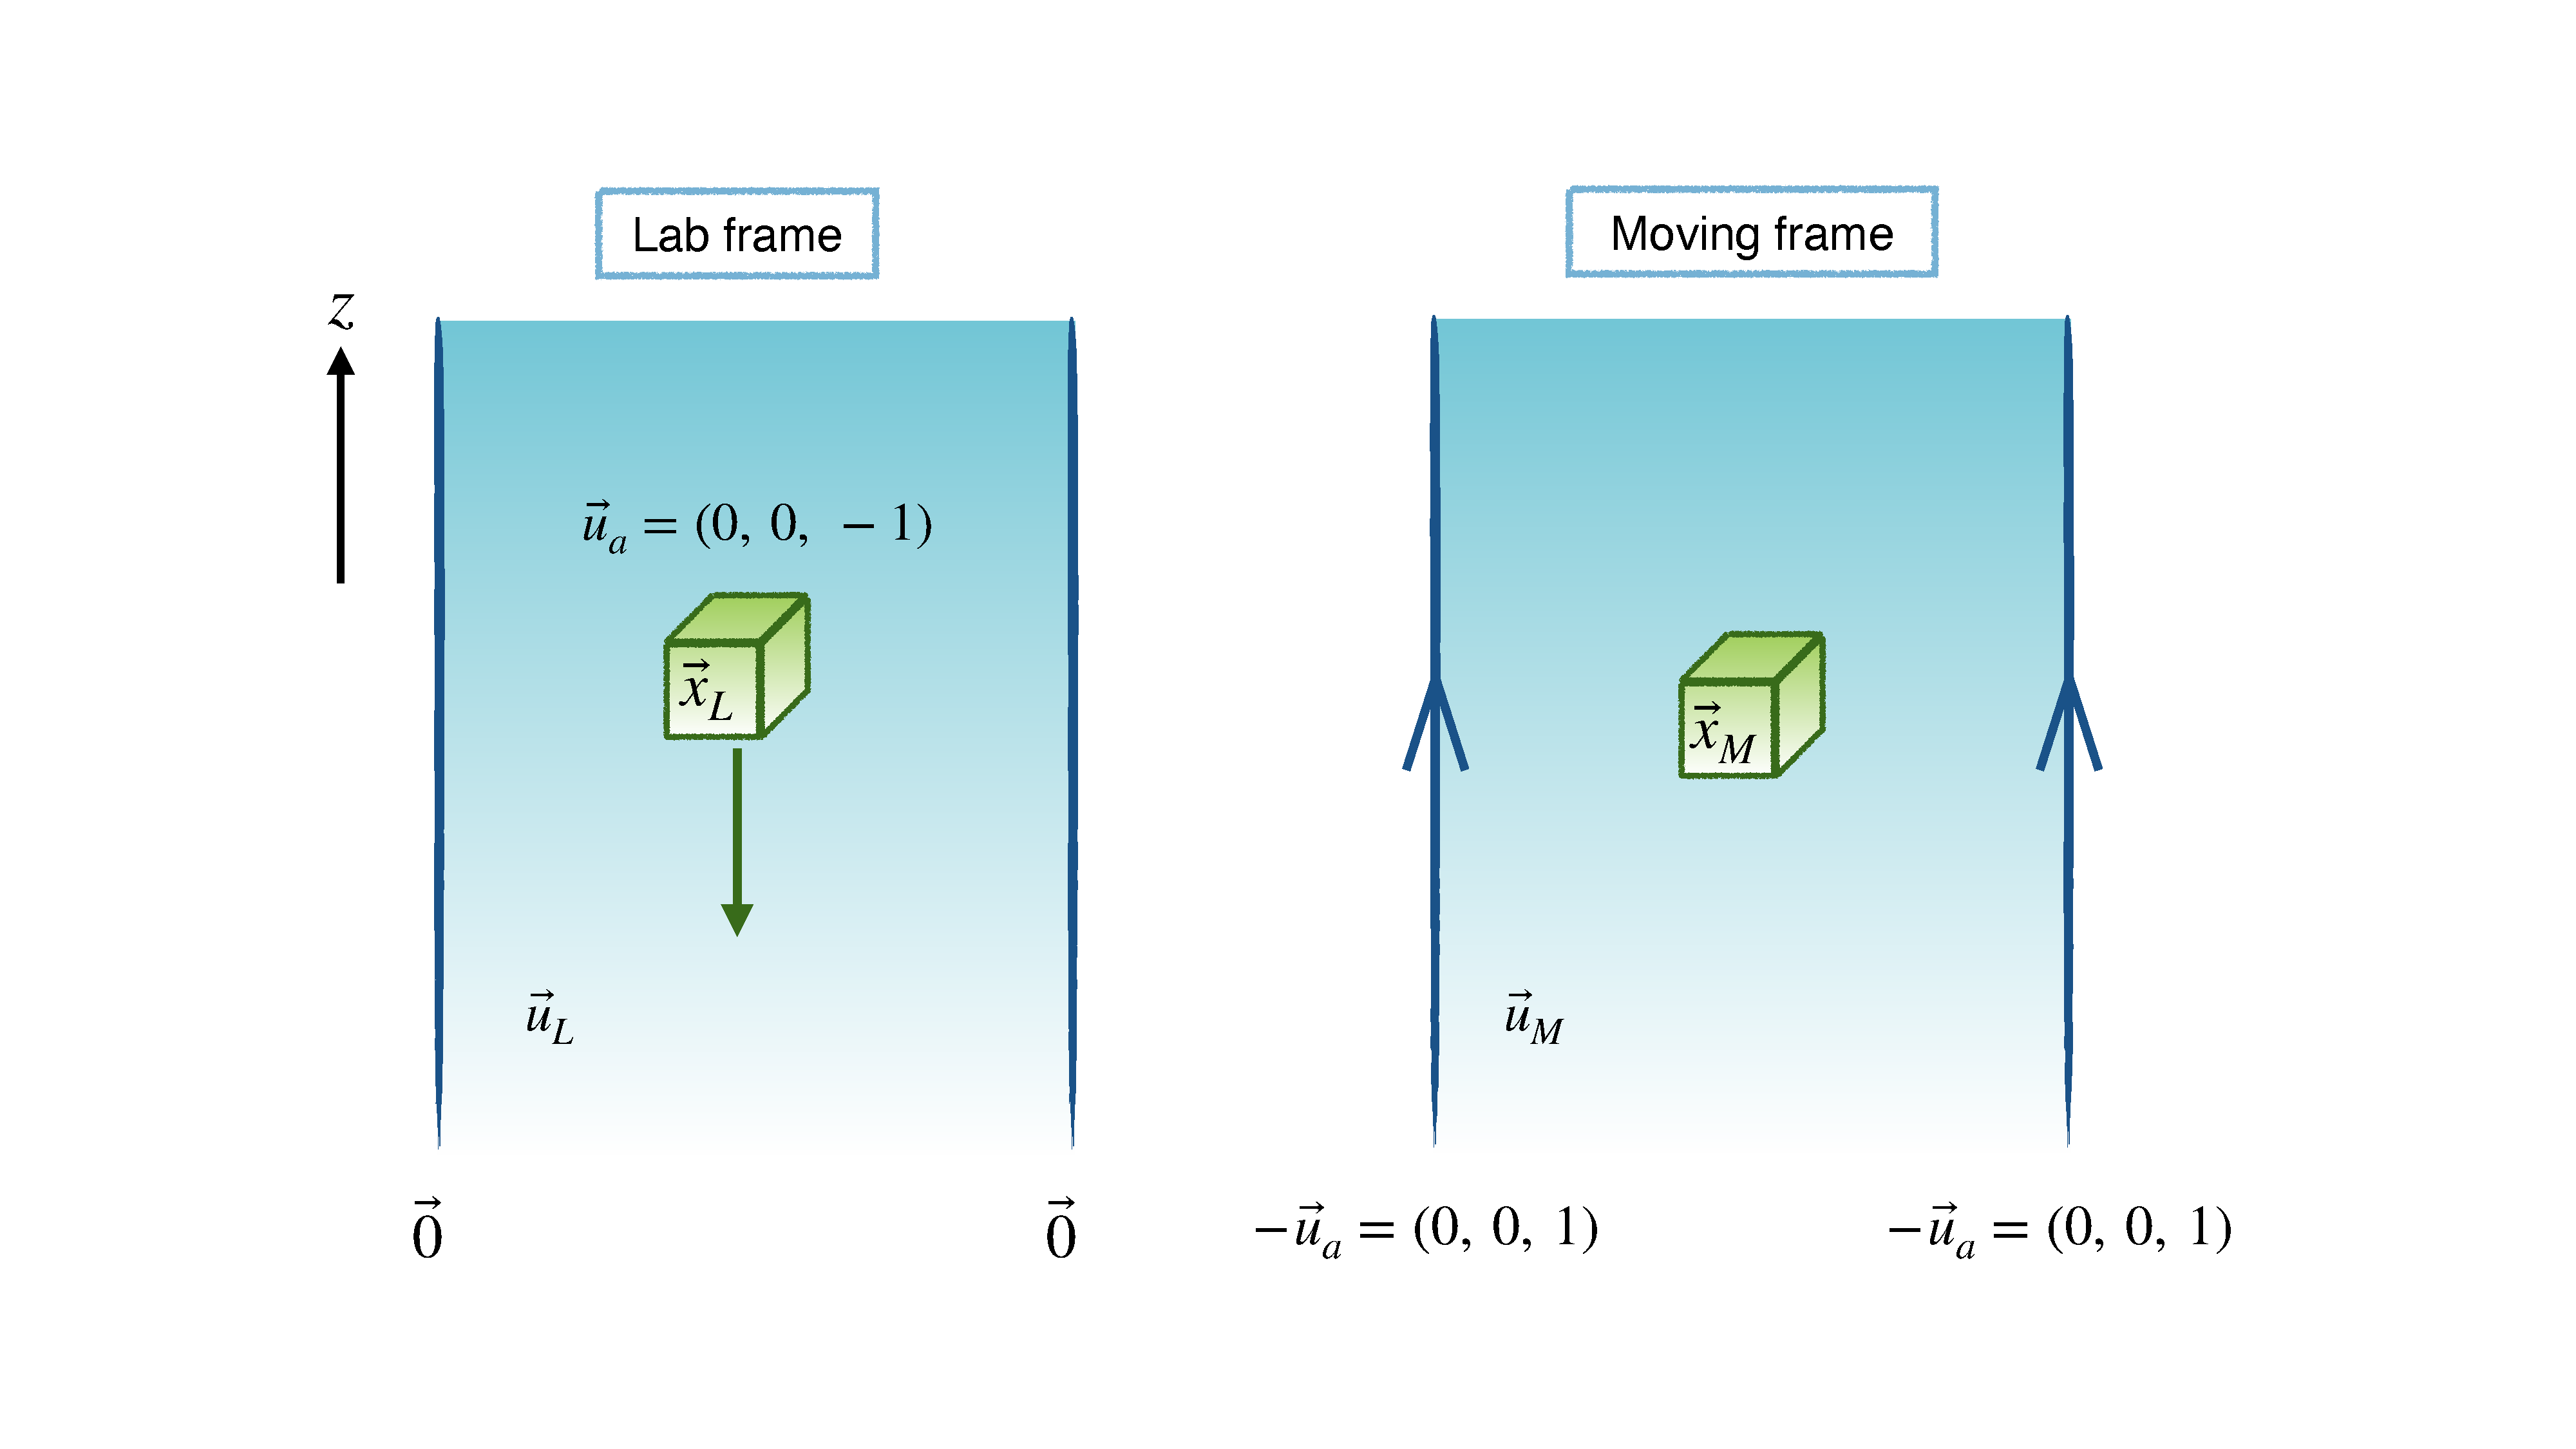
\includegraphics[scale=0.25]{figures/fig_frame_ref}
	\end{center}
	\caption{Schematics of frames of reference. (Left) lab frame and (right) moving frame of reference }
	\label{fig_frame_ref}
\end{figure}
This condition implies that the domain is large enough compared to the aggregate.
We solve for the stress on the aggregate boundary by prescribing the constant velocity or the body force of the aggregate in order to compute the fluid velocity field. 
% We then solve for the fluid equations.
% Note that the position of the aggregate at time $t$, $\vec{x}_L(t)$, can be expressed as
% \begin{equation}
% \vec{x}_L(t) = \vec{x}_L(0) + \vec{u}_s t.
% \label{eq_xl_pos}
% \end{equation}
% Note that $\vec{u}(\vec{x}, \ t)$ represents the velocity inside of the fluid domain at time $t$.
\par
On the other hand, we use the moving frame to model the concentration dynamics.
In this setting, we fix the aggregate in the middle of the fluid domain and move the fluid upward to describe the settling motion, as shown in Figure \ref{fig_frame_ref} (right).
This can be done by changing of variable from the velocities in the lab frame; we simply add $-\vec{u}_a$ to all velocities in the lab frame of reference,
\[
\vec{u}_M = \vec{u}_L - \vec{u}_a.
\]
 The velocity at the boundary of the fluid domain becomes the same speed as $\vec{u}_s$ but in the opposite direction, i.e., $-\vec{u}_a = (0, \ 0, \ 1)$. We also can see that now the aggregate has zero velocity in the moving frame of reference.

\subsection{Simulations}
As a sample simulation, we use ten cubes to model an aggregate and have discontinuous initial concentration, setting zero throughout the fluid domain, outside of the aggregate, and higher concentration inside and on the aggregate. Specifically, we prescribe values of $1$ for the inside of each cube and $0.5$ for all square faces. We also place $0.25$ and $0.125$ for all edges and corners of cubes, respectively. 
This intuitive concentration setup is to reduce the risk of any stability issue due to the discontinuity at the aggregate boundary. 

In addition to the initial concentration, the following conditions are set:
\begin{framed}
\begin{itemize}
	\item Number of cubes ($NC$) = 10
	\item Settling velocity ($\vec{U}_a$) = $(0,0,-1)$
	\item Center of mass of the aggregate ($\vec{x}_{cm}$) = $(-0.8, \  0.4, \ 0)$
	\item Maximum radius of the aggregate ($R_m$) $\approx 5.3472$
	\item Domain = $[-11.50, 9.90] \times [-10.29, 11.09] \times [-21.39, 21.39]$\\
	(Centered at the center of mass of the aggregate.)
	\item Spatial step size: $Nx = Ny = 50, Nz = 100$; $\Delta x = \Delta y = \Delta z \approx 0.43$
	\item Peclet number = 100
	\item Time step (final time = 50): $Nt = 500$; $\Delta t = 0.1$
\end{itemize}
\end{framed}

For the Peclet number we set for the sample simulation, in case it is necessary to observe a larger Peclet number that could have more numerical error, we set Pe $=100$.
We compute the fluid velocity field once using the boundary integral method and keep it fixed while we update the concentration. 
\par
We simulated this problem using both the implicit (trapezoid) and the explicit (RK2) time integration. Under the conditions provided above, we get an advection CFL condition number of approximately 0.03 and a diffusion one as 0.08. Since the CFL numbers are less than 1, we can use the RK2 method with no stability issue. 
The main reason we wanted to try the explicit method is to reduce computing time if possible. However, we found that both time integration methods gave us similar results in terms of computing time. Before we officially decide which method we are going to use for further research, we will check the order convergence.
\par
We present the snapshots of simulations using the discontinuous initial concentration in Figure \ref{fig_ic4_RK2_snap135}. It is a three-dimensional simulation; however, for clear visualization, we slice the domain at $x= -0.8$, which is the middle of $x-$axis.
 Note that we are using a moving frame of reference such that the surrounding fluid is flowing upward to represent the settling aggregate motion.
After time $t \approx 30$ in Figure \ref{fig_ic4_RK2_snap135}, we can see lower concentration is going outside of our numerical domain.  
 \begin{figure}[h]
 \begin{center}
	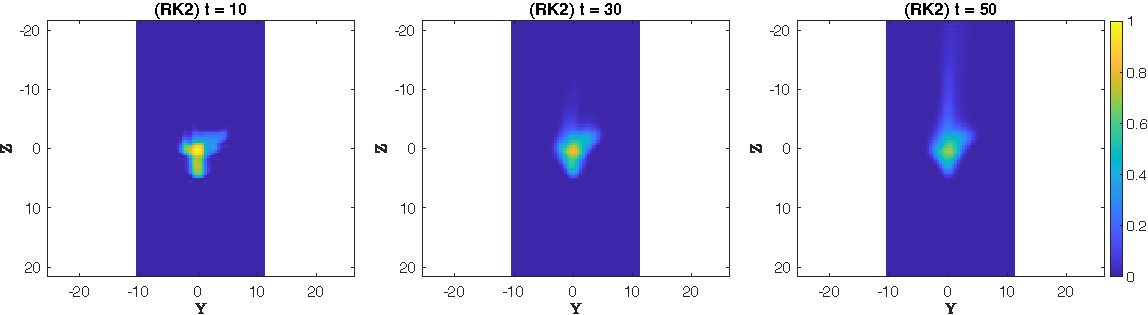
\includegraphics[scale=0.75]{./figures/fig_ic4_RK2_snap135}
 \end{center}
 \caption{Discontinuous initial concentration with finite differences space and RK2 time schemes.}
 \label{fig_ic4_RK2_snap135}
 \end{figure}
 
Figure \ref{fig_sumC} shows the sum of the concentration of the fluid over time.
The results seem to be consistent with our expectation that the mass is conserved until the flow reaches the upper boundary of our domain. The right plot in Figure \ref{fig_sumC} shows the concentration difference between each time and the initial one up to time $t = 20$. This can be interpreted as a perturbation, which increases over time.  
 \begin{figure}[ht]
 \begin{center}
    \epsfig{figure=./figures/fig_sumC_ic4_only.eps, scale = 0.3}
	%  \hspace{5mm}
	\epsfig{figure=./figures/fig_sumC_error_ic4_only.eps, scale = 0.3}
 \end{center}
 \caption{(Left) Variation of total concentration in the fluid domain in time. (Right) The error between the total concentration at each time and the initial sum of concentration.}
 \label{fig_sumC}
 \end{figure}
 %% -------About the Concentration Dynamics here --------------------------------
 \subsection{Discussion}
 
 There are several topics we can study further with the homogeneous ambient fluid case. We may continue analyzing the preliminary results for the dissolved CO$_2$ model we presented.
 As an application of the dissolved CO$_2$ simulation, we consider the remineralization of marine aggregates. In particular, We can apply a method of remineralization and model dissolved CO$_2$ of marine aggregates in order to study the carbon flux profile in a homogeneous fluid.
 In a recent article, Omand {\it{et al}} \cite{omand_sinking_2020} proposed a derivation of the sinking particle flux model with a sphere.
 %{FB}
 Several aspects of this derivation can be improved with a model such as ours and we can provide justifications for features that were assumed or roughly estimated.
  With our randomly shaped aggregate model, we expect to present more accurate dynamics and could calculate the size of a sphere with equivalent diffusive properties as a function of aggregate size and fractal dimension.
%   This analysis can be done with the code we have written. 
%    I will participate in this study for providing the code and producing figures. The work will be done mainly by my advisors, Blanchette and Khatri.
 %
 %---------begin conclusion here from the agg. paper ---------------------------
\section{Conclusion}
\label{sec:conclusion}

We have developed a novel implementation of boundary integral methods for flow around aggregates composed of cubes. In this case, we found that the single-layer approach was more accurate and therefore used it to study the flow around randomly formed aggregates.
We have presented the results of the flow around individually-added aggregates and cluster-to-cluster aggregates and characterized the resulting forces on the aggregates. We have identified a suitable length scale to characterize the behavior of fractal aggregates in various contexts. To describe the drag or force, and torque, on an aggregate, the gyration radius, $R_g$, is the best choice, with respective scalings of $\vec{F} \sim \tilde{\mu} \vec{U}_a R_g$ and $\vec{Q} \sim \tilde{\mu} \vec{\Omega} R_g^3$, as should be expected in Stokes flow. 
An improved collapse of the drag is possible if we account for an aggregate's departure from its typical size, $\bar{R}_g$, through the factor $\sigma_g = \frac{R_g - \bar{R}_g}{\bar{R}_g}$. 
The nearly linear relationship between the drag and the gyration radius indicates that the choice of $R_g$ to describe the size of an aggregate is an appropriate one while, for example, the volume-based size $L=V^{1/3}$ would not yield a linear relationship with the drag.  



We have also considered the effects of extensional flow on aggregates, an aspect that has been understudied. We introduced a simple characterization of the straining force, $\vec{E}$, on a solid object. We used computations of the straining force to determine that the maximum radius, $R_m$, is the most appropriate length scale to predict the impact of extensional flow on an aggregate and found that $\vec{E} \sim \tilde{\mu} |\lambda| R_m^2 \hat{v}$. This is particularly relevant when considering aggregate formation and break up. As in the case of the force, an improved collapse
of straining force is 
possible using an aggregate's departure from its typical size, $\sigma_m = \frac{R_m - \bar{R}_m}{\bar{R}_m}$. 


Our numerical approach can be directly applied to compute the flow around several particles. We thus plan to use it in future work to conduct a more accurate investigation of aggregate formation. In the present study, as is the case in the vast majority of diffusion-limited aggregation studies, aggregates were formed without factoring in flow dynamics. Our numerical approach allows us to determine the response of the system dynamically when subjected to stochastic forces. Rather than assuming a constant drag and no deformation, we may instead calculate the forces acting on every particle, determine the deformation or potential break-up of the particles by matching the viscous stress with the particle's elastic stress, and determine the aggregates settling velocity as it deforms. Such an approach should provide the most accurate aggregate formation model yet, which in turn will allow for a more accurate characterization of their properties.

Another promising avenue for future work is the incorporation of stratification effects. Marine aggregates typically settle in a water column where the density increases with depth, owing to salinity and temperature variations. Since aggregates are very porous, they are sensitive to stratification \cite{prairie_delayed_2013}. 
Fluid entrainment and diffusive effects play a role to first stopping, and then restarting the settling of the porous aggregate
\cite{panah_simulations_2017}. This process has already been modeled using spherical particles, but how diffusion affects fractal-like aggregates remains unclear. By coupling the current simulations to a concentration field subject to advection-diffusion and tracking its effect on the particle density, one should be able to obtain a simple but improved approximation of the behavior of aggregates settling in a stratified ambient. Our approach may also be extended, though with a significant increase in computational effort, to account for the effects of stratification on the flow itself by adding a volume integral of the concentration to the equation (\ref{eq_slp}), thus providing a complete picture of the effects of density stratification.

